\documentclass[journal]{IEEEtran}
%\documentclass[conference]{IEEEtran}
\IEEEoverridecommandlockouts
\usepackage{cite}
\usepackage[cmex10]{amsmath}
\usepackage{graphics}
\usepackage{graphicx}
\usepackage{subfigure}
\usepackage{epsfig}
\usepackage{algorithmic}
\usepackage[linesnumbered,ruled,slide]{algorithm2e}
\usepackage{amsfonts}
\usepackage{float}
\usepackage{enumerate}
\usepackage{verbatim}
\usepackage{caption3}
\usepackage[justification=centering]{caption}
\usepackage{epstopdf}
\usepackage{url}
\usepackage{array,subfig}

\begin{document}
\pagestyle{empty}
\thispagestyle{empty}

\title{DroneLoc: Drone Localization with Smartphone Camera Network\vspace{-1mm}}

%\author{\IEEEauthorblockN{Naigao Jin, Lei Wang��Xingwen Zhang, Wei Liu, Qing Tan }\\
%\IEEEauthorblockA{School of Software, Dalian University of Technology, China\\
%Key Laboratory for Ubiquitous Network and Service Software of Liaoning Province\\
%ngjin@dlut.edu.cn}
%\thanks{Naigao Jin is the corresponding author.}
%\vspace{-2mm}}

% make the title area
\maketitle

%\thispagestyle{plain}
%\pagestyle{plain}
\pagestyle{empty}
\thispagestyle{empty}


\begin{abstract}
%\boldmath
Drones are increasingly flying in sensitive airspace where their presence may cause harm, such as near airports, forest fires, large crowded events, secure buildings, and even jails. A cost-effective drone detection and localization system is needed to warn of the presence of drones in such cases. Unpredictable computer controlled movements, speed and maneuver abilities of drones, their resemblance to birds in appearance when observed from a distance make it challenging to detect, identify and correctly localize them in complex outdoor environments. 
To overcome these limitations in existing costly solutions, this paper formally describes, designs, implements, and evaluates a smartphone-based  drone  localization system, i.e., DroneLoc.
The key idea behind DroneLoc is to utilize the classify ability of deep neural network  to implement drone detection, then implement drone localization by fusion the detection result of multiple smartphones.
In this study, we investigate camera integrated in modern smartphone and leverage the location in the image as measurement information.
DroneLoc  turns the localization problem into search problem  by collecting the  detection data of smartphones in the camera network. 
Location in the image is estimated through  deep neural network . 
Drone localization is performed by minimizing the  distance between the measured sequence and the vectors in a database.
The proposed DroneLoc system is evaluated through extensive simulations and physical experiments (a test-bed with 30 smartphone nodes). 
Evaluation results demonstrate that ThunderLoc can effectively localize the drone with good robustness.
\end{abstract}

\begin{IEEEkeywords}
Drone Localization, Camera Network
\end{IEEEkeywords}

\IEEEpeerreviewmaketitle


\section{Introduction}
%DroneLoc

With the advent of inexpensive commercially available un-manned aerial vehicles (UAV), drones are rapidly rising in popularity as a host of a wide class of applications ranging from commercial delivery , environment monitoring, photography, policing, fire fighting, just to name a few. However, with the rise in drone usage, there has also been a rise in incidents involving drones, such as mid-air collisions, damage to property, and violations of privacy.
In particular, drones are increasingly flying in sensitive airspace where their presence may cause harm, such as near airports, forest fires, large crowded events, and even jails. A quadcopter crashed on the White House lawn, raising concerns about the safety of buildings and political leaders. The presence of drones has interfered with and grounded aircraft fighting forest fires. Drone crashes have also disrupted sporting events such as the US Open tennis tournament as well as a World Cup skiing race. In fact, based on FAA data, more than 300 drone incidents were reported in California alone between April 2014 and Jan 2016, which is equivalent of 15 incidents per month on average or 1 incident every two days.

A variety of approaches have been explored to interdict drones. 
These include shooting nets at the drones to tamper with their propeller to bring them down, using lasers to shoot down drones, spoofing GPS to confuse a drone localization system, hijacking the software of drones by hacking into them, using other drones to hunt down unauthorized drones, and even training eagles to attack and disable drones. 
However, these interdiction strategies typically presume that the presence of the drone has already been detected. 
Geofencing is useful to prevent drones from flying into fixed areas known a priori as sensitive, but requires manufacturers to install such software and is less useful to prohibit drones from flying around temporary event venues. The work utilizing passive RF to identify drones has sought, for example, to detect the frequency of transmission, the MAC address of the drone, and the frequency of packet communication. 
Recent work has sought to develop drone detection systems that leverage either microphone, camera, or radar to sense the presence of drones. Considering the physical signatures of the drone motion, Mobisys2017 detect the presence drone by passively eavesdropping on the RF communication between a drone and its controller (Wi-Fi standard). 
All these techniques suffer from various limitations. Audio-based approaches can be confused by other sounds in noisy environments, has limited range, and cannot detect drones that employ noise canceling techniques. Thermal and IR imaging cameras for long distance are prohibitively expensive and have limited coverage. Radio-frequency techniques based on active radar introduce RF interference. RF-based methods often mistake the drone for birds and increase nuisance alarm rate.

In this paper, we propose a new method for thunder localization by leveraging dual-microphone smartphones.
With commodity dual-microphone smartphones, the binary left/right data from dual-microphone of each smartphone is effectively
collected and utilized to estimate the location of the thunder.
The proposed system solely relies on the collaborative effort of the participating users to achieve thunder localization.
The ThunderLoc project created such a prototype system with different types of Android based mobile phones, and validate our approach with a virtual thunder study, showcasing the potential of the proposed solution. 
DroneLoc  takes advantage of the sensing capabilities, including the acoustics, position and orientation offered by the microphone, GPS, accelerometer and magnetometer on the smartphones.
The key idea of DroneLoc is the division of a 2D localization space into distinct regions by the perpendicular bisectors of lines joining dual-microphone in each smartphone. 
Each distinct region formed in this manner can be uniquely identified by a binary sequence.
We firstly construct the binary sequence table that maps all these feasible binary sequences to the corresponding regions by using the locations and directions information of the smartphone nodes.
The smartphone nodes determine the measured binary sequence based on the sign of TDOA between two microphones of each smartphone node.
The location of an acoustic source is estimated by searching through the binary sequence table to determine the ��nearest�� feasible sequence to the measured sequence. 
To our knowledge, drone localization with smartphone-based  has not been considered in the literature before.
Our contributions are as follows:

1) We designed, implemented, and deployed a smartphone-based
drone localization system called
DroneLoc. Our DroneLoc app for Android platform has
been installed by more than 1,00 smartphone in our
university to monitor the drone near our campus. To the
best of our knowledge, DroneLoc is the first smartphone-based drobe localization service.




The rest of the article is organized as follows. Section \uppercase\expandafter{\romannumeral 2} presents an overview of the DroneLoc system.
Then, the design of ThunderLoc is introduced in section \uppercase\expandafter{\romannumeral 3}.
Section \uppercase\expandafter{\romannumeral 4} discusses several issues concerning practical system deployment.
Section \uppercase\expandafter{\romannumeral 5} presents simulation results and an empirical evaluation on
the test-bed. Section \uppercase\expandafter{\romannumeral 6} briefly surveys related work.
Section \uppercase\expandafter{\romannumeral 7} concludes the whole article.







\section{System Overview}


% GPS, accelerometer,magnetometer and gyroscope
 The ThunderLoc system architecture was designed to allow transmission of data from dual-microphone smartphones to the cloud platform with crowdsensing mechanism.
 %Most of smartphones have dual-microphone which provide hardware supports for our paper.
 ThunderLoc leverages stereo recording with high sampling rate of off-the-shelf mobile devices to estimate the left/right binary information.
 The perpendicular bisector of dual-microphone divides the localization space into two regions.
 If the thunder is on the right of the perpendicular bisector, then the binary code of the corresponding half-plane is set as 1, 
 and the code of the left half-plane is set as 0.


  \begin{figure}[htb]
            \setlength{\abovecaptionskip}{0pt}
            \centering
            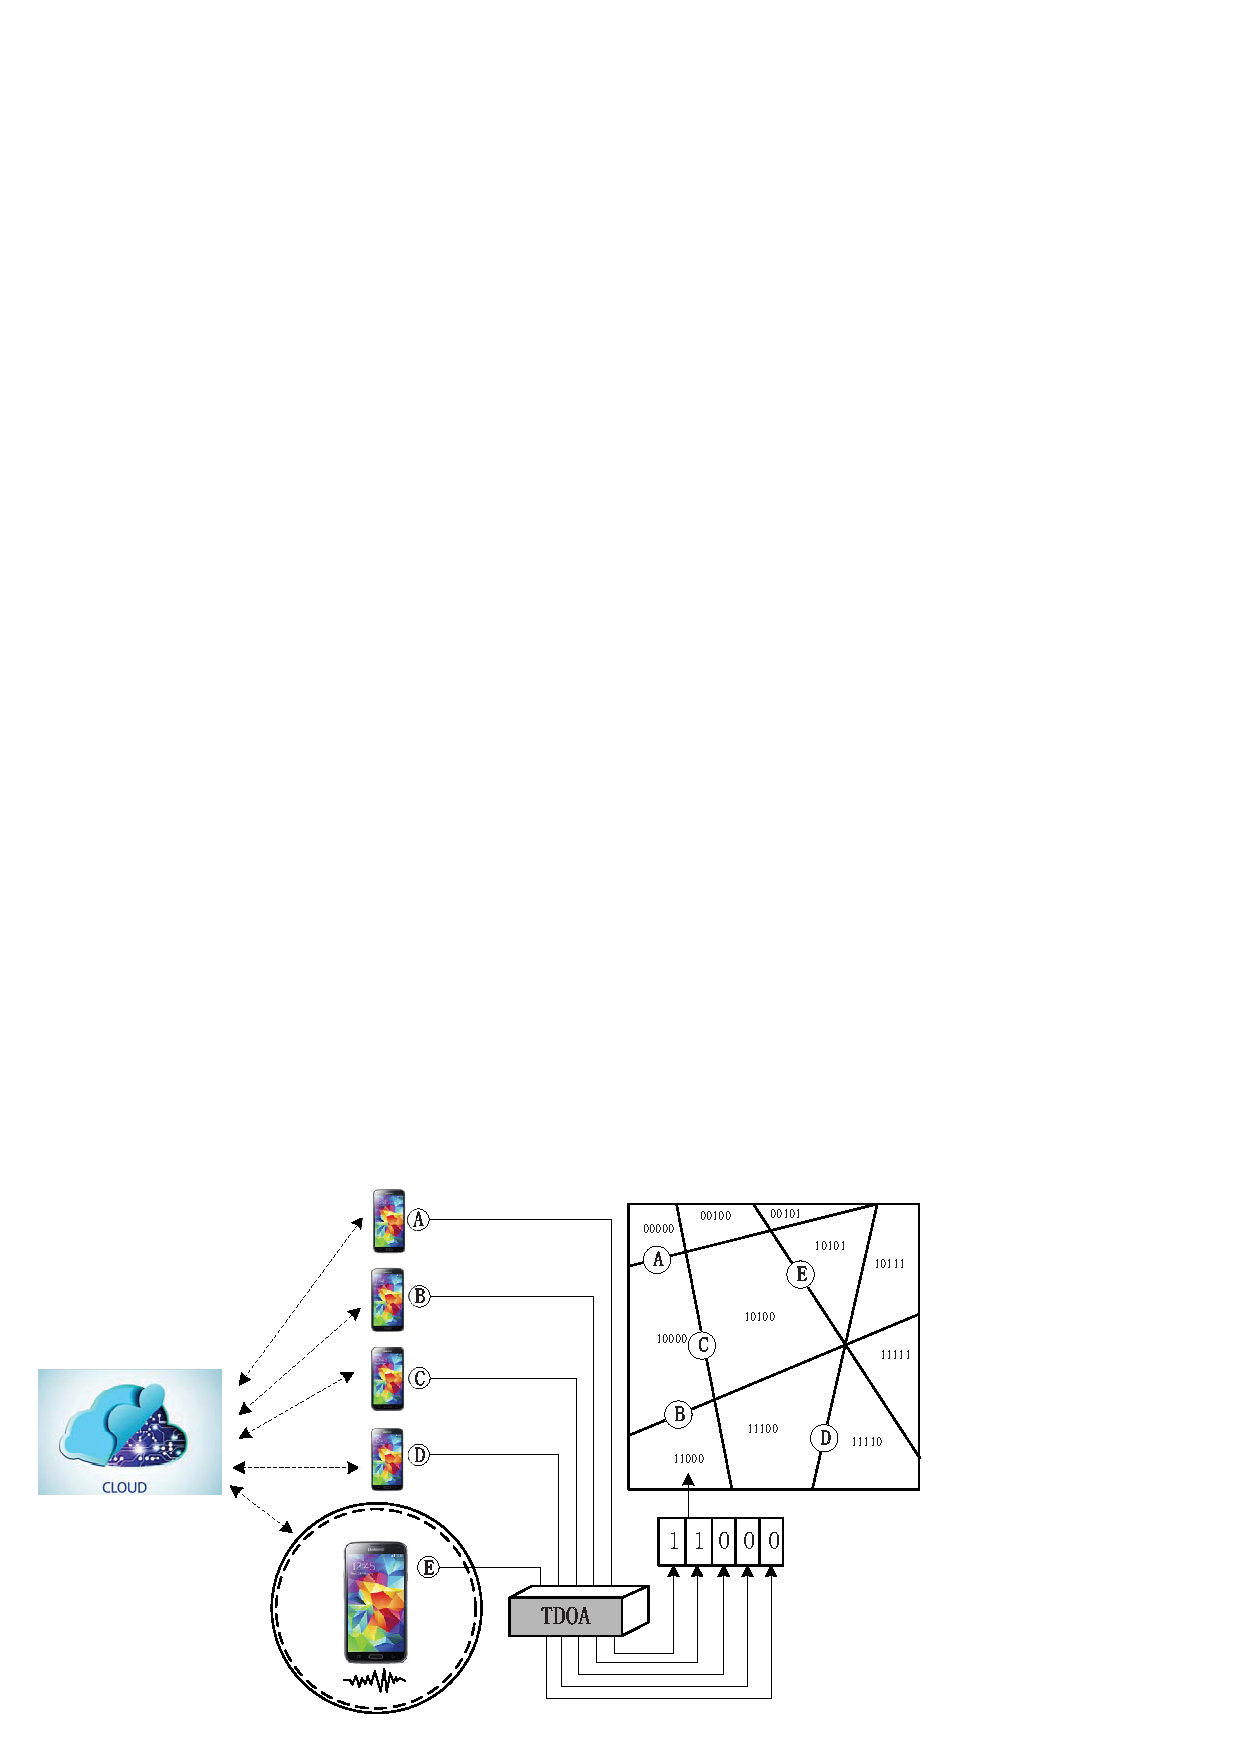
\includegraphics[scale=2,height=5.0cm]{fig/overview.pdf}
			 \vspace{1mm}
            \caption{\label{overview}System overview.}
            \vspace{-4mm}
  \end{figure}
  
 Fig. \ref{overview} shows a layout of ThunderLoc system.  
 This research involves the use of dual-microphone smartphones as a ad-hoc sensor array based on crowdsensing in 4G cellular mobile network,
  To simplify the problem, an 2D localization space consisted of $N$ dual-microphone smartphones is considered,
 and the signals acquired by the dual-microphone of the same smartphone are synchronized.
 The perpendicular bisectors of  $N$ dual-microphones divide the localization space into some small subregions.
 
 In this paper, the thunder localization problem can be solved by using the map information and the measured binary sequence.
 Briefly, the ThunderLoc system works as shown in Fig. \ref{architecture}. 
 In the client end, the location information and direction information of the smartphone can be estimated by GPS and the motion sensors (such as accelerometer, gyroscope) integrated in the smartphone, respectively.
 When a thunder occurs, each smartphone detects TDOA of two synchronized signals recorded by dual-microphone, then achieves the binary left/right data according to the sign of TDOA.
 The APP in each smartphone uploads the binary measurement data, the location information and direction information of the smartphone to the cloud computing platform together.
 During the data collection, participants can be even unaware of the collection task in which they are actually involved.
 Besides, ThunderLoc encourages participants to manually upload the sensing data to cloud computing platform when they hear the thunder.
 Thunder localization algorithm is run on the cloud computing platform to localize the dominant thunder.
With these random distributed smartphones, the area can be divided into subregions, according to the positions and directions of the smartphone nodes.
This naturally gives a N-vector binary codes called the detection binary sequence in cloud computing platform,
as shown in Fig. \ref{overview}, which embedded relative position relationships among the smartphone nodes and the thunder. 
With the pre-computed subregion division, the location of the thunder can be estimated by processing the binary detection sequence.
   \vspace{-4mm}
  \begin{figure}[htb]
            \setlength{\abovecaptionskip}{0pt}
            \centering
            \includegraphics[scale=2,height=5.0cm]{fig/architecture.pdf}
			 \vspace{1mm}
            \caption{\label{architecture}System architecture.}
            \vspace{-4mm}
  \end{figure}
  
In the next section, we will provide the basic ThunderLoc system firstly, 
then the robust version of ThunderLoc is proposed to deal with the adverse condition in the practical application scenario.
  








\section{DESIGN}

ThunderLoc adopts the client-server system architecture to allow transmission of data from the mobile devices to a server station or cloud platform.
When a thunder occurs, the smartphones will be triggered to transmit their positions, directions and binary measurement data to the server. 
The server will subsequently process the received data to implement thunder localization. 
In this section, we firstly introduce the design of client application, then two localization methods in the server end are introduced in the next two subsections.
  \vspace{-3mm}
\subsection{Data collection on client end}
  \vspace{-0mm}
  
Screen shots of the application and visualizations
used by the participants of the thunder can be seen in
Fig. \ref{Screen}. Fig. \ref{Dual}. shows the two channel sound signals from dual-microphone in a mobile phone.
It is easy to see that the thunder firstly reaches the microphone that corresponding to the top channel.

  \begin{figure}[hptb]
            \setlength{\abovecaptionskip}{0pt}
            \centering
            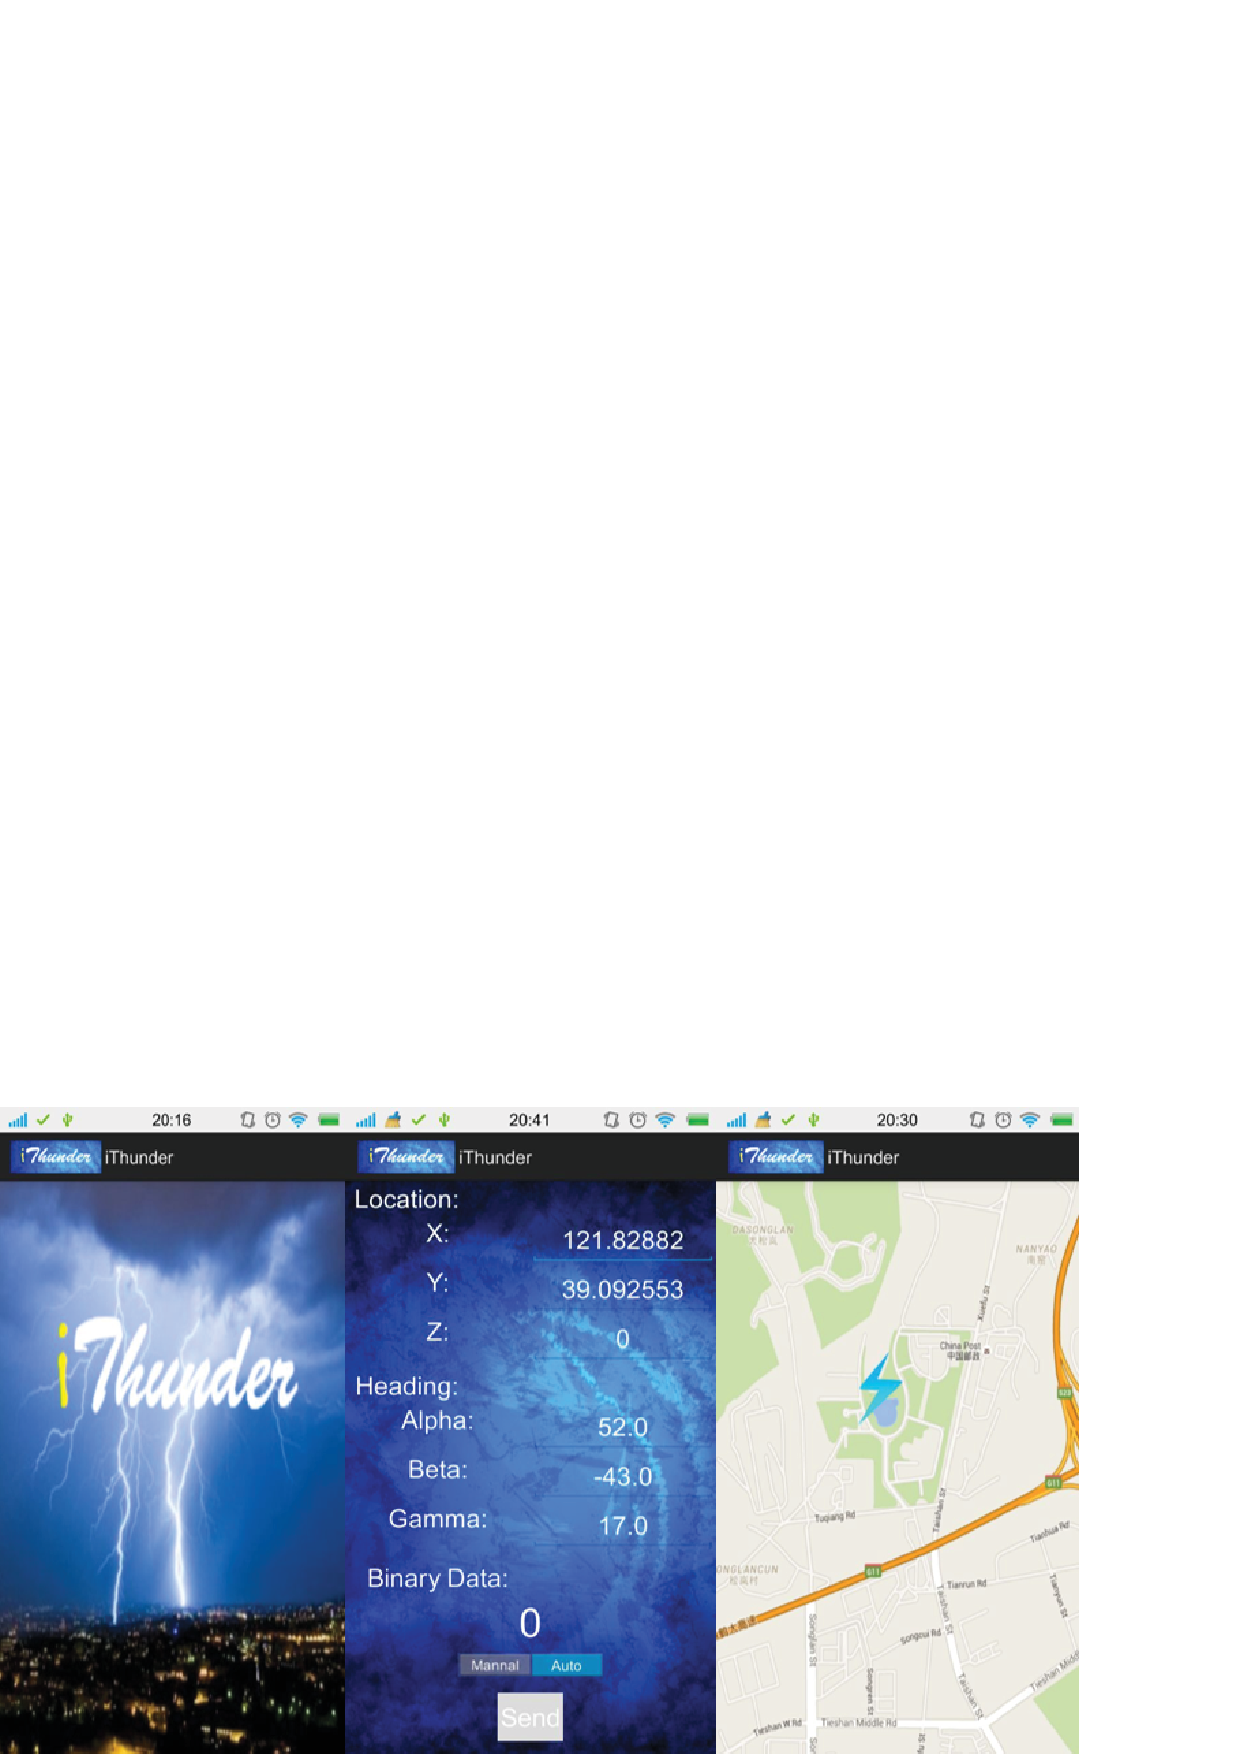
\includegraphics[scale=1.4,height=4.0cm]{fig/ThunderLoc.pdf}
			 \vspace{4mm}
            \caption{\label{Screen}Screen shots of ThunderLoc client application.}
            \vspace{-6mm}
  \end{figure}
  
  

  \begin{figure}[ht]
            \setlength{\abovecaptionskip}{0pt}
            \centering
            \includegraphics[width=9cm,height=4cm]{fig/dualmic.pdf}
     \vspace{2mm}
            \caption{Dual-microphone acoustic signals.}
            \label{Dual}
            \vspace{-2mm}
  \end{figure}



  \begin{figure}[ht]
            \setlength{\abovecaptionskip}{0pt}
            \centering
            \includegraphics[scale=2,width=6.0cm]{fig/client.pdf}
     \vspace{2mm}
            \caption{The diagram of signal processing of acoustic signals.}
            \label{Diagram}
            \vspace{-4mm}
  \end{figure}



Fig. \ref{Diagram} depicts the flow of the ThunderLoc client application. 
ThunderLoc client application has two main independent threads: sensing thread and
communication thread. The sensing thread handles the interaction
with the main application and the on-board sensors, the communication thread
handles local storage, transmission of recorded sensor events and requeues of events in the case of poor network connection. 
Considering the energy problem, it is not an energy-effective solution for the mobile devices to continuously send
data to the servers. To deal with this issue, a three-state model is
used for ThunderLoc client application: Idle Mode, Listening Mode and Communication Mode. 
Fig. \ref{Mode} depicts the different modes of sensing of the client end.
While continuously recording and sensing for probable thunder events locally on the mobile phones, this model permits minimal transmission of data to the server. 
 

  \begin{figure}[ht]
            \setlength{\abovecaptionskip}{0pt}
            \centering
            \includegraphics[scale=1.4,height=4.0cm]{fig/modechange.pdf}
     \vspace{4mm}
            \caption{Modes of sensing of the client end}
            \label{Mode}
            \vspace{-4mm}
  \end{figure}


1) Idle Mode:
In order to determine the orientation of a mobile phone, the mobile device must be stationary for a period of time while recording the sensor data. 
Device movement is characterized by a change in the readings of the accelerometer and gyroscope. 
If the cumulative movement is under the threshold, the device will be verified as still, then jumps into the listening mode.

2) Listening Mode:
Thunder is the acoustic shock wave resulted from a sudden and intense heating of the air in the lightning channel. 
%The application is able to capture the shock wave by always keeping recoding a
%segment of the signal in a circular memory buffer before the threshold triggering of the system. 
The system is triggered when a shock wave above a predetermined threshold is recorded. 
Specially, the trigger is fired when an average energy is rising 4 times experienced by any of
the dual microphones. 

3) Communication Mode: To reduce the total latency of the ThunderLoc system, it is necessary to transmit data as soon as possible after
a thunder event occurs. 
The application records sensor readings about heading and location of the smartphone, then immediately transmits these data to the server along with the binary measurement data estimated from two channel acoustic signals of dual microphones.
In case the communication service is not available during the thunder event, a copy of these recordings is stored locally, then placed into a queue to be sent once communication is available again.

Besides the implicit way to collect data, 
ThunderLoc also allows user to explicitly input location, 
direction and binary measurement data by the way of `humans as sensor'~\cite{wang2014using}. %~\cite{wang2014using,resch2013people}

%~\cite{wang2014using,resch2013people}.



 
  \vspace{-1mm}
\subsection{Basic localization on server side}
  \vspace{-0mm}
  
    \begin{figure}[ht]
            \setlength{\abovecaptionskip}{0pt}
            \centering
            \includegraphics[scale=1.4,height=4.0cm]{fig/server.pdf}
     \vspace{4mm}
            \caption{The diagram at cloud platform.}
            \label{Server}
            \vspace{-4mm}
  \end{figure}

  
In this section, the position and orientation of a smartphone are assumed to be known, which can be estimated by its GPS(or Wi-Fi based indoor localization) and motion sensors, respectively.
Fig. \ref{Server} depicts the flow of the ThunderLoc server application. In the cloud computing platform, the map of space division can be built with the position and orientation information of all smartphone nodes.
Then, we can turn the acoustic source localization into the searching problem in the Hamming space. 

Firstly, we introduce the basic localization method. Let us consider the 4G network with $N$ dual-microphone smartphones randomly deployed in 2D area. 
The top-level idea for basic ThunderLoc is to split the whole localization area into some subregions identified by respective binary sequences.
Given $N$ smartphone nodes in the localization space, the whole number of combinations of binary sequences is $2^N$ in theory.
However, in the practical system, given $N$ smartphone nodes in the localization space,
the possible number of combinations of binary sequences is only $(N^2+N+2)/2$.
The lower dimensionality of the sequence table enables the correction of errors in the measured sequence.
This is one of the reasons that our proposed algorithm performs well in adverse conditions.
Localization system can achieve higher localization performance as the number of smartphones increases, such extensibility is an unique advantage compared with dedicated microphone array hardware.



\textbf{Binary sensor model}:
 We propose a binary sensor model, where the TDOA of dual-channel acoustic signals is converted reliably to one bit of information: the thunder is on the left or right of the perpendicular bisector of dual-microphones. 
We use the sign of TDOA as 1 bit measurement information, which reveals the left/right information about the direction of the incoming Thunder.
Using 1-bit measurement information allows for inexpensive sensing as well as minimal communication load.
As shown in Fig. 2, for each dual-microphone smartphone node, 
TDOA is computed by traditional time delay estimation method (such as generalized cross correlation, GCC), % ~\cite{knapp1976generalized}
then we can get the binary sequence of the thunder.

  \begin{figure}[ht]
            \setlength{\abovecaptionskip}{0pt}
            \centering
            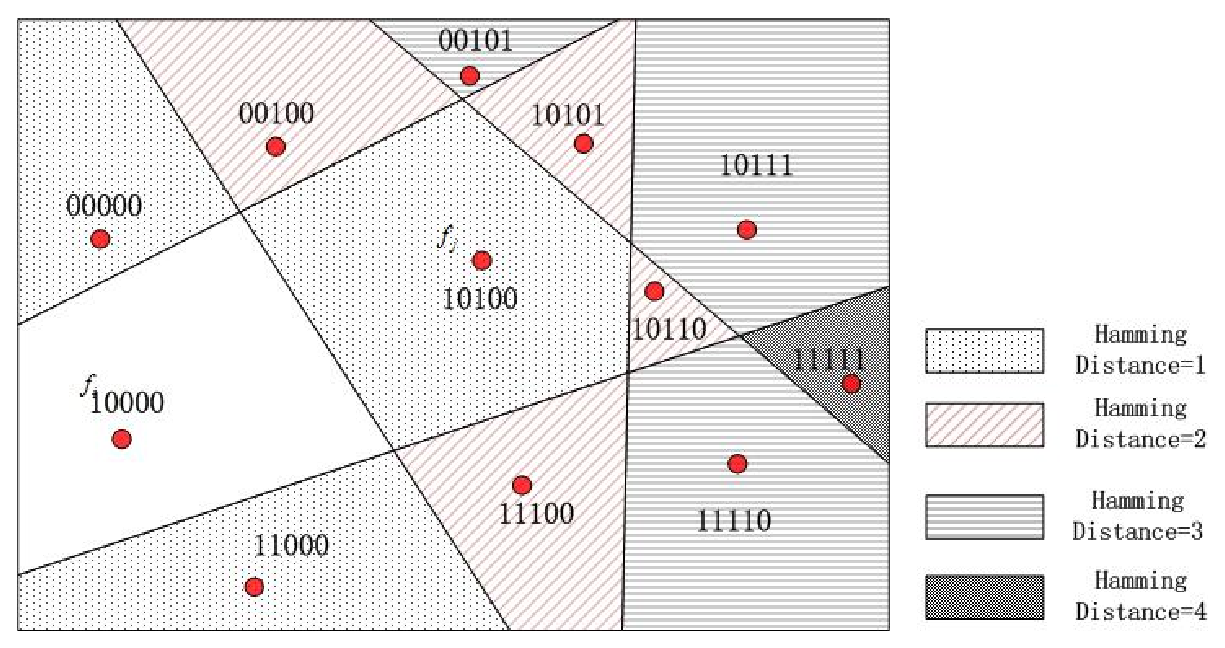
\includegraphics[scale=1.4,height=4.0cm]{image/Hamming_distance2.eps}
     \vspace{4mm}
            \caption{Hamming distance vs. geographic distance.}
            \label{Hamming}
            \vspace{-8mm}
  \end{figure}

\textbf{Hamming distance}:
For two faces $f_i$ and $f_j$ in Fig. \ref{Hamming}, now there are two types
of distance: (i) the geographical distance $GD({f_i},{f_j})$ between the center points of ${f_i}$ and ${f_j}$, and (ii) the Hamming distance
$HD({f_i},{f_j})$. Hamming distance measures the number of dimensions where two vectors have different values. 

  
  
\begin{figure}[hptb]
 \setlength{\abovecaptionskip}{0pt}
	\begin{minipage}[t]{0.45\linewidth}
		\centering
		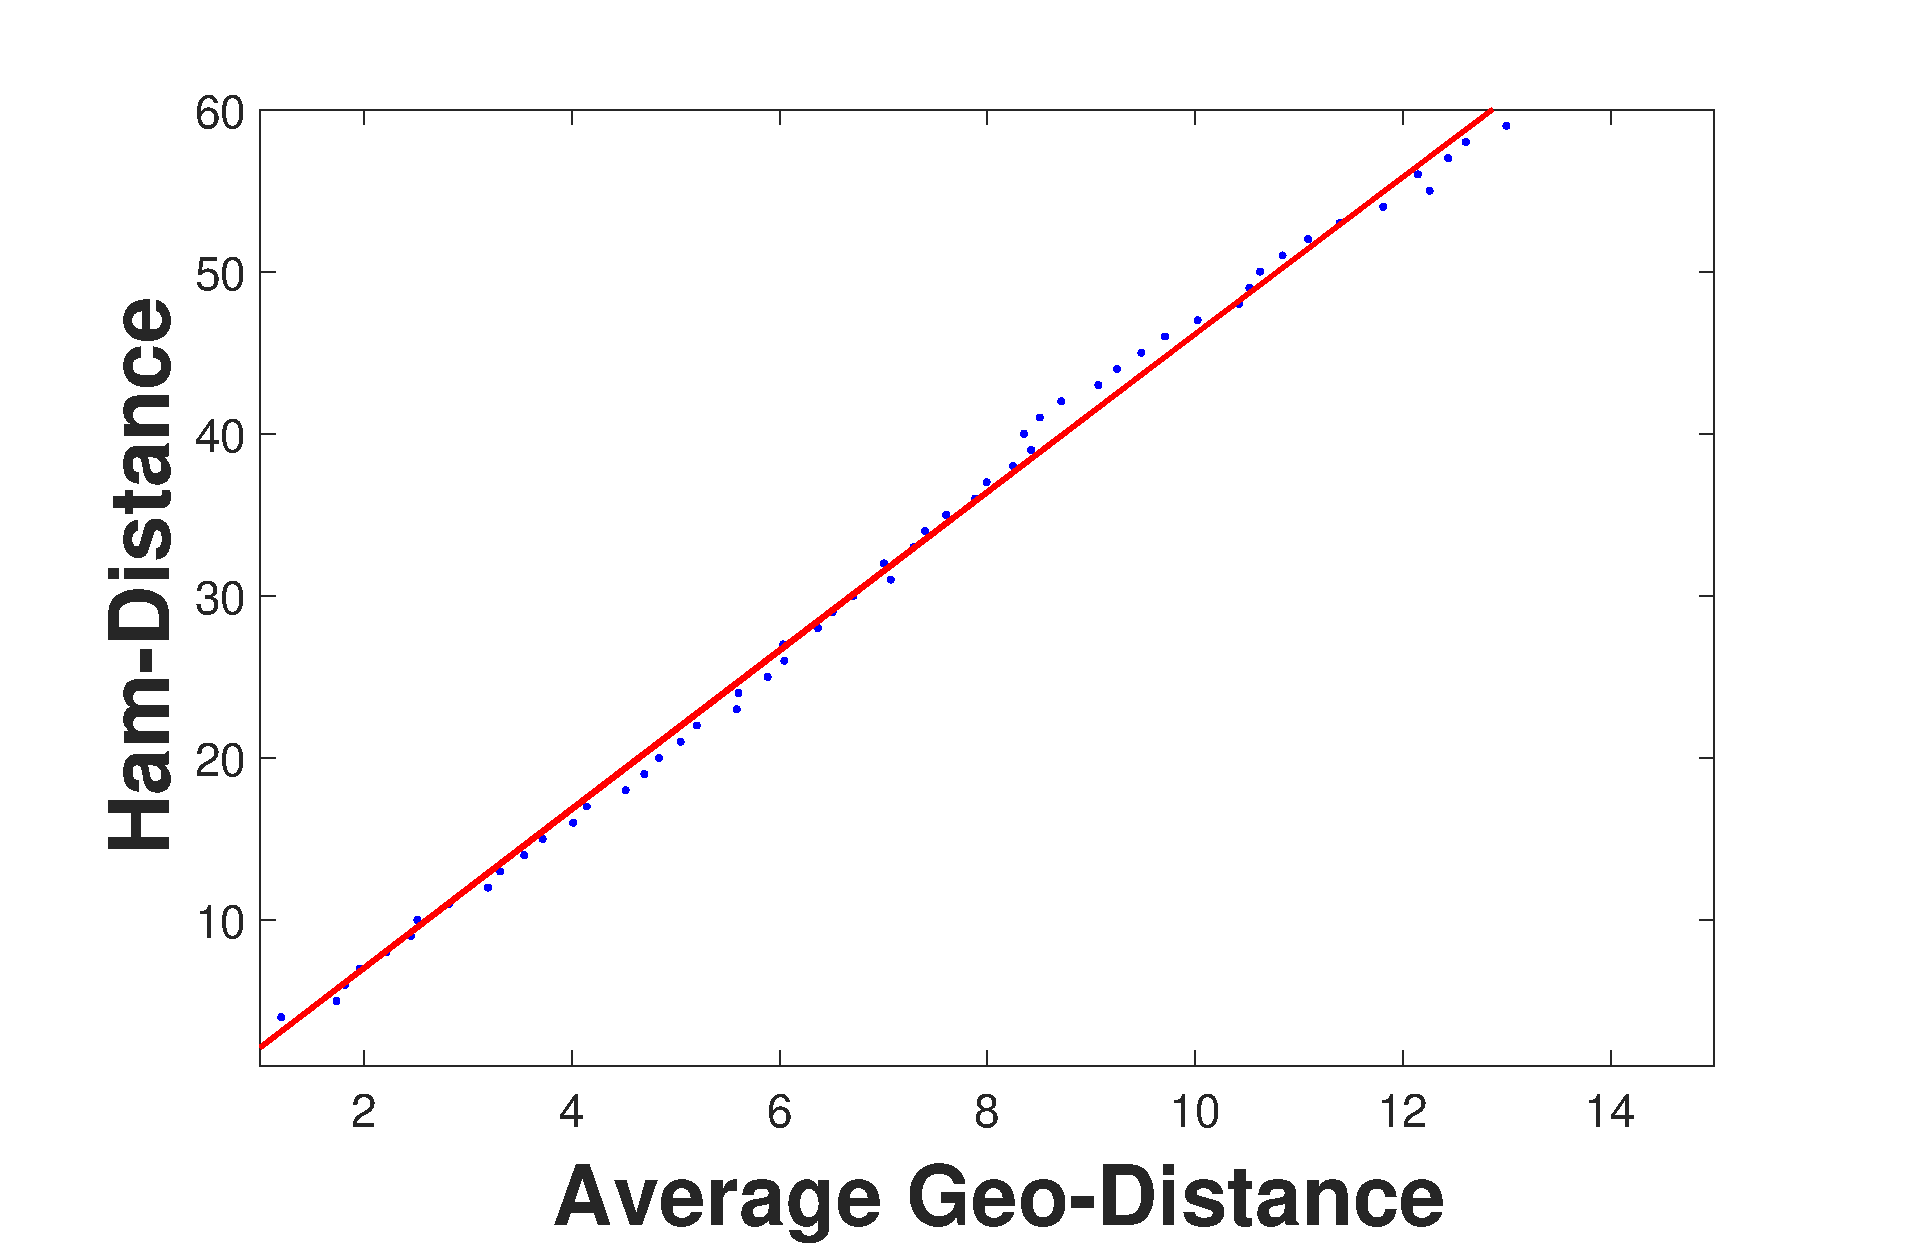
\includegraphics[height=2.85cm]{fig/Hamming1.eps}
		 \vspace{2mm}
	%	\caption{Hamming distance vs. Average geographic distance.}
	\vspace{-2mm}
	\end{minipage}%
		\hspace{1mm}
	\begin{minipage}[t]{0.45\linewidth}
		\centering
		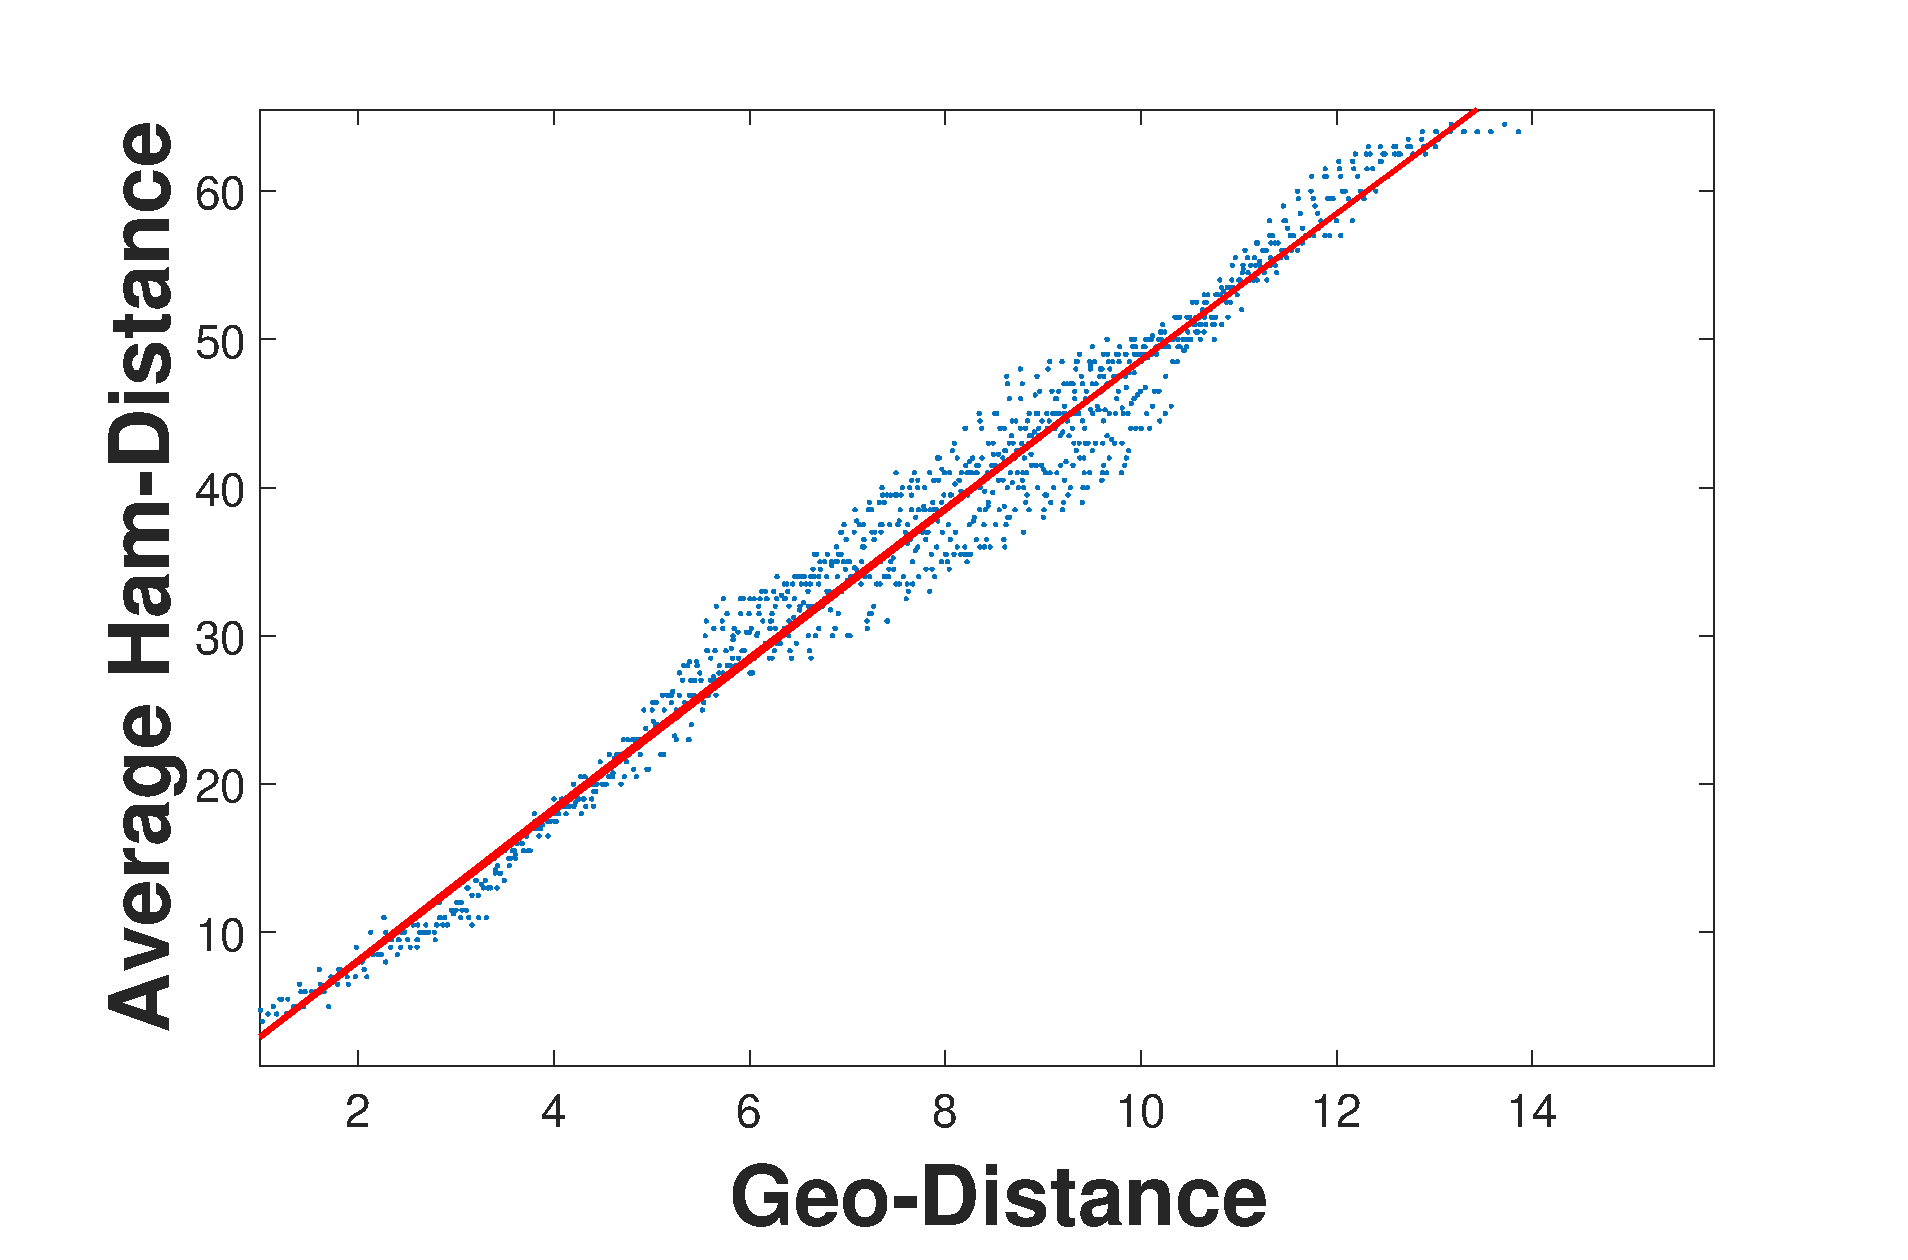
\includegraphics[height=2.85cm]{fig/Hamming2.eps}
		 \vspace{4mm}
	%	\caption{Average Hamming distance vs. Geographic distance.}
		\vspace{-4mm}
	\end{minipage}	
				\vspace{1mm}
			\caption{Relationship between Hamming distance and geographic distance.}
			\label{relationship}
		\vspace{-6mm}		
\end{figure}		
		
%  \ref{fig1} : ��figure��table���ƣ������У���д\caption{}��д\label{}��
From Fig. \ref{relationship} we can see that
the closer the two faces are in geographical distance, the smaller their Hamming distance is.
In other words, geographical distance is positively correlated with Hamming distance.  
For these two distances, we have the following observation:
 \begin{equation}
  \label{equation.1}
GD({f_i},{f_j}) \propto HD({f_i},{f_j})
 \end{equation}
 
Equation \eqref{equation.1} indicates that the Hamming distance between
two faces is approximately proportional with their geographical
distance. This is because longer geographical distance creates
more chances to cross bisectors, resulting in more flipped bit.  
So when the Hamming distance is close to zero, then the locations are very close to each other.  
Moreover, we do lots of simulation experiments to prove it. 
The result of the experiments can be seen in Fig.7 and Fig.8. It proves that Hamming distance is almost linear growth with geographical distance increasing. 
Given a query binary vector from multiple smartphones, we can estimate the location by retrieving the vectors in the beforehand database
and find the smallest Hamming distance. 
In other words, we can find the target location through by querying the smallest Hamming distance.



The basic ThunderLoc contains the three steps:

(1) Dividing the space into $p$ grid points : Suppose there is an acoustic source at the point $P{_i},i=1,...,p$, the $j-th$ smartphone $n{_j},j=1,...,N$ can compute the TDOA and get the sign of the TDOA.
Then we can get the binary code $C{_i,_j} \in \{ 0,1\}$ by the sign of TDOA. 
Combining the binary code of all $N$ smartphones, we can get a N-vector binary sequence $D{_i},i=1,...,p$. 
The database about $p$ discrete points is obtained, and an item in the database is ${S_i} = \{ D_i, P_i\} $.

(2) Computing the binary sequence $T$ of the target: When the acoustic source emits sound, 
all the smartphone nodes compute the TDOA, then get the sign of TDOA and determine the binary code. 
$ TDOA_{i}$  of the $ i-th $ smartphone can be computed by using time delay estimation algorithm(such as GCC), 
and the binary code of the ${i-th}$ smartphone can be defined by computing the sign of the TDOA:
 \begin{equation}\label{eq:eps}
Binary\_data_{i}=
\left\{\begin{matrix}
1 ,~~ $if$~~  TDOA_{i}\geq0;\\
0 ,~~ $if$~~  TDOA_{i}<0.
\end{matrix}\right.
 \end{equation}

(3) Processing the binary sequences $T$: Computing the Hamming distance between $T$ and each $D(i)$, the acoustic source position can  be found by searching the minimum of Hamming distance. However, it should be noted that in general there are several source points with the same
minimum value of Hamming distance. 
This is due to the finite estimate resolution which creates areas with the same Hamming distance. 
The final position estimate is the mean of all points with the minimum Hamming distance.  

We can calculate time complexity according to the three steps.
In step 1, we build the database, including calculating TDOA of a pair of microphones and getting its sign just use the linear time.
For each grid point we need to calculate TDOA of $N$ pairs of microphones and there exists $P$ grid points, so the time complexity in step 1  is $O \left( {PN} \right)$.
The time complexity of step 2 is $O \left( {N} \right)$ similarly.
In step 3, the time complexity of the search processing is  $O \left( {PN} \right)$. So the overall time complexity is $O \left( {PN} \right)$.

	
\begin{figure}[ht]
	\setlength{\abovecaptionskip}{0pt}
	\begin{minipage}[t]{0.45\linewidth}
		\centering
		\label{fig:subfig:a}		
		\includegraphics[height=2.8cm]{image/node.eps}
		\vspace{2mm}
		\subfigure{(a)}
		%\subfigure{(a) Measurement error.}
		\vspace{-2mm}
	\end{minipage}%
\hspace{0.5cm}
	\begin{minipage}[t]{0.45\linewidth}
		\centering
		\label{fig:subfig:b}
		\includegraphics[height=2.8cm]{image/angleposition.eps}
		\vspace{2mm}
		\subfigure{(b)}
		%\subfigure{(b) Angle error and position error.}
		\vspace{-4mm}
	\end{minipage}	
	\vspace{1mm}
	\caption{The impact of variety of errors.}
	\label{Impact}
\end{figure}		
		
	\vspace{-4mm}
  
The bit flip problem for measurement data and the location and direction parameter errors have impact on the localization performance as shown in Fig. \ref{Impact}.
As shown in Fig. \ref{Impact}$(a)$, In case the measurement binary data from node B is flipped, the binary sequence $'10'$ is turned into $'11'$, reducing the accuracy of localization system. 
In Fig. \ref{Impact}$(b)$, if the position measurement or angle measurement of sensor B is inaccurate, 
there is a certain distance between actual position and estimated position.
According to the above, the basic Thunderloc is not suitable for the practical application. In the next section, 
we propose a robust localization solution against the measurement errors, position errors and orientation errors of smartphones.

  
\vspace{-4mm}
\subsection{Robust localization on server side}

In the practical application, the bit-flip problem mentioned before should be considered.
Moreover, the measurement error and  the uncertainty of node parameters have effects on the localization performance.
In this subsection, the robust version of ThunderLoc is devised to circumvent these problems.
The results we have obtained empirically indicate that the robust localization method can dramatically reduce the localization error under the practical application.

In order to improve the robustness of the localization system, the possible coordinates for the thunder are computed through selecting the K smallest Hamming distance instead of the minimum Hamming distance. 
Then, the centroid estimation method is utilized to set the center of gravity of  all the possible points as the estimated location of the thunder.

However, the selection of  the parameter $K$ is a difficult task. Deeply thinking the relation between the Hamming distance and the 2D geographic distance, the smaller Hamming distance is, the closer the coordinate region is to the target.
For each discrete point in localization space, the weight of each coordinate point is assigned based on Hamming distance.
Specially, the weight of each coordinate point is monotonic decreasing function of Hamming distance.

Gaussian function is adapted to weight discrete points according to the respective Hamming distance:
\begin{equation}
\label{weight}
{w_i} = exp(-HD(T,D_i)/N{\sigma ^2})
\end{equation}
where $\sigma$ is the parameter to decide the weighting strategy. 

Based on the normalized weight $\bar {w_i}$, the final estimated location of the thunder is estimated by computing the weight sum of all grid points:
\begin{equation}
 \label{normalized}
{\bar w_i} = \frac{{{w_i}}}{{\sum\limits_{i = 1}^P {{w_i}} }}
\end{equation}

\begin{equation}
 \label{estimated}
\hat x = \sum\limits_{i = 1}^P {{{\bar w}_i} \cdot {p_i}}
\end{equation}

Algorithm \textbf{1} illustrates the pseudo code of robust ThunderLoc method.
\begin{algorithm}
\caption{Robust ThunderLoc}
 \textbf{Input:} The location coordinates of all smartphones \\
\quad \quad \quad  The orientations of all the smartphones \\
\quad \quad \quad  Information about microphones $measure\_data$ \\
\textbf{Output:} Location of the thunder\\

\textbf{Step 1:} Database building:\\
\textbf{Step 2:} Computing the binary code $T$ of the thunder from the dual-channel acoustic signals: \\
\textbf{Step 3:} Processing the binary sequence: \\

(1) Computing Hamming distance for each point:\\
\For{$i \leftarrow 1$ \textbf{to} $p$}
 {
 ${HD(T,D(i))} = \sum\limits_{j = 1}^N {\left( {{T}(j) \oplus {D_i}(j)} \right)}$
 }
 
(2) Computing the weight of each grid point using Eq. \ref{weight} :\\
(3) Normalizing the weights and Estimating the source location using Eq. \ref{normalized} and  Eq. \ref{estimated}, respectively.\\
\end{algorithm}

%\vspace{-4mm}
Compared with the basic ThunderLoc, robust ThunderLoc leverages all possible points to locate the thunder.
Although the computing load increases, robust ThunderLoc has two benefits: (i) Avoiding the problem of selecting parameter $K$; (ii) More robust to measurement errors and node parameter errors.
Our evaluation in sections \ref{section:results} shows that robust localization method considerably enhances the robustness of localization system.

We can calculate time complexity of robust ThunderLoc according to the three steps. 
From the algorithm we can see  the time cost is the same as basic localization method in step 1 and step 2.
Besides, in step 3, we should calculate the normalized weighting of each point, and the corresponding time complexity is $O\left({P} \right)$.
At last step, we should calculate the location of the thunder by the weight sum of each grid point, and the corresponding time complexity is $O\left({P} \right)$.
The time complexity of robust ThunderLoc method is also $O\left( {PN} \right)$.
At the cost of $O\left({P} \right)$ time complexity more than basic ThunderLoc method, robust ThunderLoc method enhances system robustness.
The computing of Hamming distance is the core of the proposed ThunderLoc system, 
which can be effectively implemented via the Boolean XOR operation in the cloud computing platform with GPU and FPGA support.




\section{Discussion}

\subsection{Humans as sensors}

Humans as sensors defines a new measurement model for crowdsensing. In the model, measurements are
not only taken by smartphone, but also come from the personal observations of participants. 
As a complement of automatically acquiring the localization data from smartphones, ThunderLoc provides the interface for participants to manually upload personal observations.
The users of smartphones can manually input the personal localization data in the ThunderLoc app, 
including the binary left/right data, the position and direction when they hear the thunder.

However, how to motivate enough participants for ThunderLoc is a problem in reality. 
%The incentive mechanisms for smartphone collaboration are out of range of the paper. 
Here a possible solution is given as follows. ThunderLoc app can be integrated into a weather forecast app. When the thundershower is coming, 
the weather forecast app pushes a notice to inquire whether the user to join the ThunderLoc project. 
If the user agrees to participate in, ThunderLoc app will be downloaded and run. Once the cloud platform finishes the localization operation,
the position of thunder will be push to the user. 
The well-informed discussions about the incentive mechanisms for smartphone collaboration are detailed in Ref.~\cite{duan2012incentive}.


\subsection{The impact of background noises}
Above, we put forward basic ThunderLoc and robust ThunderLoc to implement thunder localization by using dual-microphone smartphones.
The binary left/right measurement data of each smartphone is from the sign of TDOA between two audio signals recorded with dual-microphone. 
However, in the practical localization system, bit flip problem may occur because of the effect of background noises in the phase of computing binary left/right for each smartphone,
then lead to localization error.

%In the presence of background noise, 
%some of the peaks in related to reflective paths might have a magnitude that turns out to be comparable to or larger than that of the direct path. 
%For this reason, we use the reliability index that computes the ratio between the energy in a window containing the highest peak and the energy of the remaining samples in GCC-PHAT:

%\begin{equation}
%F(i) = \frac{{\sum\nolimits_{\tau  \in W} {R_{m_i^1,m_i^2}^2}(\tau ) }}{{\sum\nolimits_{\tau  \notin W} {R_{m_i^1,m_i^2}^2} (\tau )}}
%\end{equation}
%where $W$ is an interval around the highest peak in the GCC-PHAT algorithm.

\iffalse
  \begin{figure}[ht]
            \setlength{\abovecaptionskip}{0pt}
            \centering
            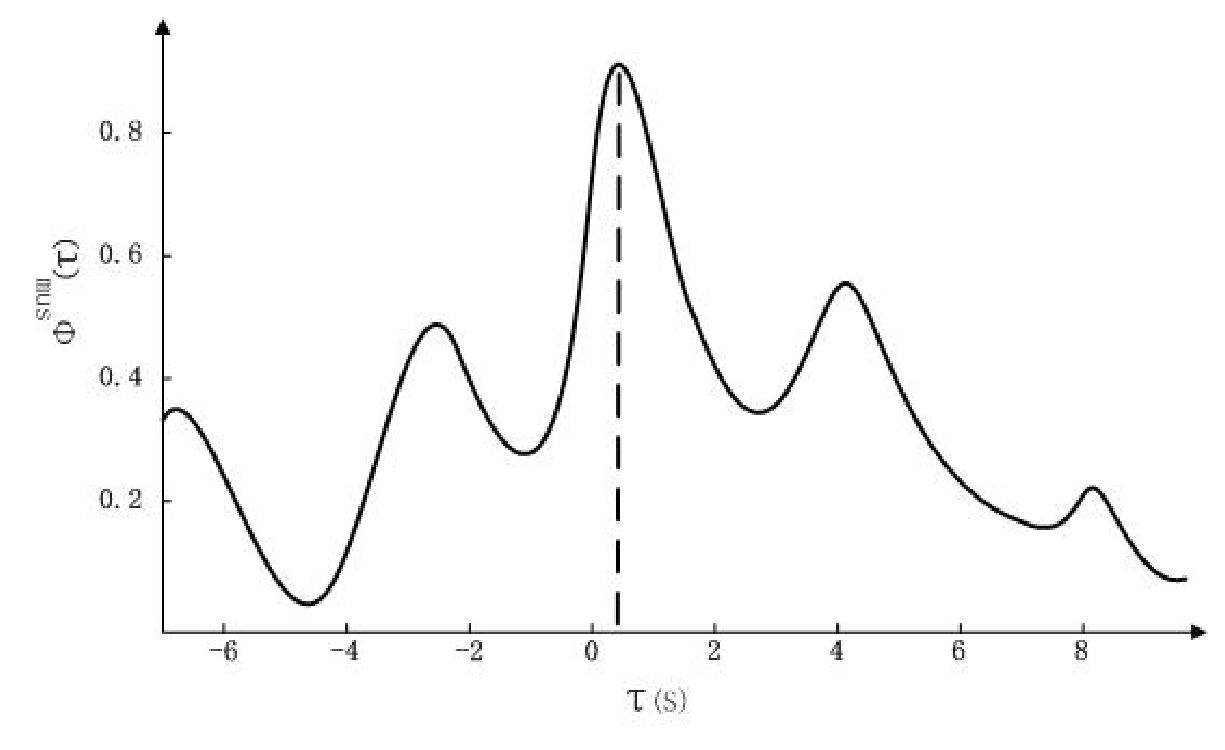
\includegraphics[scale=1.4,height=4.0cm]{image/tde.eps}
            \caption{weight calculation.}
            \label{weighting}
            \vspace{-1mm}
  \end{figure}
  \fi

%when TDOA is bigger, the result of 1 bit quantization is more reliable. 
The lower SNR is, the measurement of this smartphone is more unreliable.   
We use the SNR of each smartphone node as the reliability metric, then compute Hamming distance with the reliability information.

The new localization method is the same as robust localization method described in Algorithm \textbf{1}, 
the only difference is that using of the weighting Hamming distance instead of traditional Hamming distance:

\begin{equation}
WHD = \sum\limits_{i = 1}^N {F(i) \left( T(i) \oplus D_j(i)\right)}
\end{equation}


\subsection{System scalability and multiple thunder localization}
 Our system is evaluated in the small campus area, but it can extend to large area. The Fig.11 describes system scalability. 
In Fig.11, the signal from thunder in large-scale system only can cover limited area which means when we measure the binary sequence, 
 just a small portion of microphones close to the thunder are effective. 
 So the binary sequence of thunder is shorter than N (there exist N dual-microphone smartphones). 
We can use a range R to put the large-scale system down to a smaller area which is large enough to cover the coverage of the thunder's signal. 
And the small area can be handled as our algorithm proposed by preceding part of the paper. 
By this way, the length of the binary sequence is shorter and matching is more efficient.


Localizing multiple, simultaneously active acoustic sources is a more difficult task. 
In order to avoid conflict of several acoustic sources, 
multiple source localization must be able to uniquely identify the signature of each thunder, 
which is beyond the capability of this paper, and we will not do too much discussion about it in this paper. 
For example, if the several thunders are set as shown in Fig. \ref{multiple_source_localization},
we can calculate the positions of the two thunders because the thunder I is far enough from thunder II. 
The smartphones close to effective area I could handle thunder I, and another smartphones close to effective area II could handle thunder II. 

  \begin{figure}[ht]
            \setlength{\abovecaptionskip}{0pt}
            \centering
            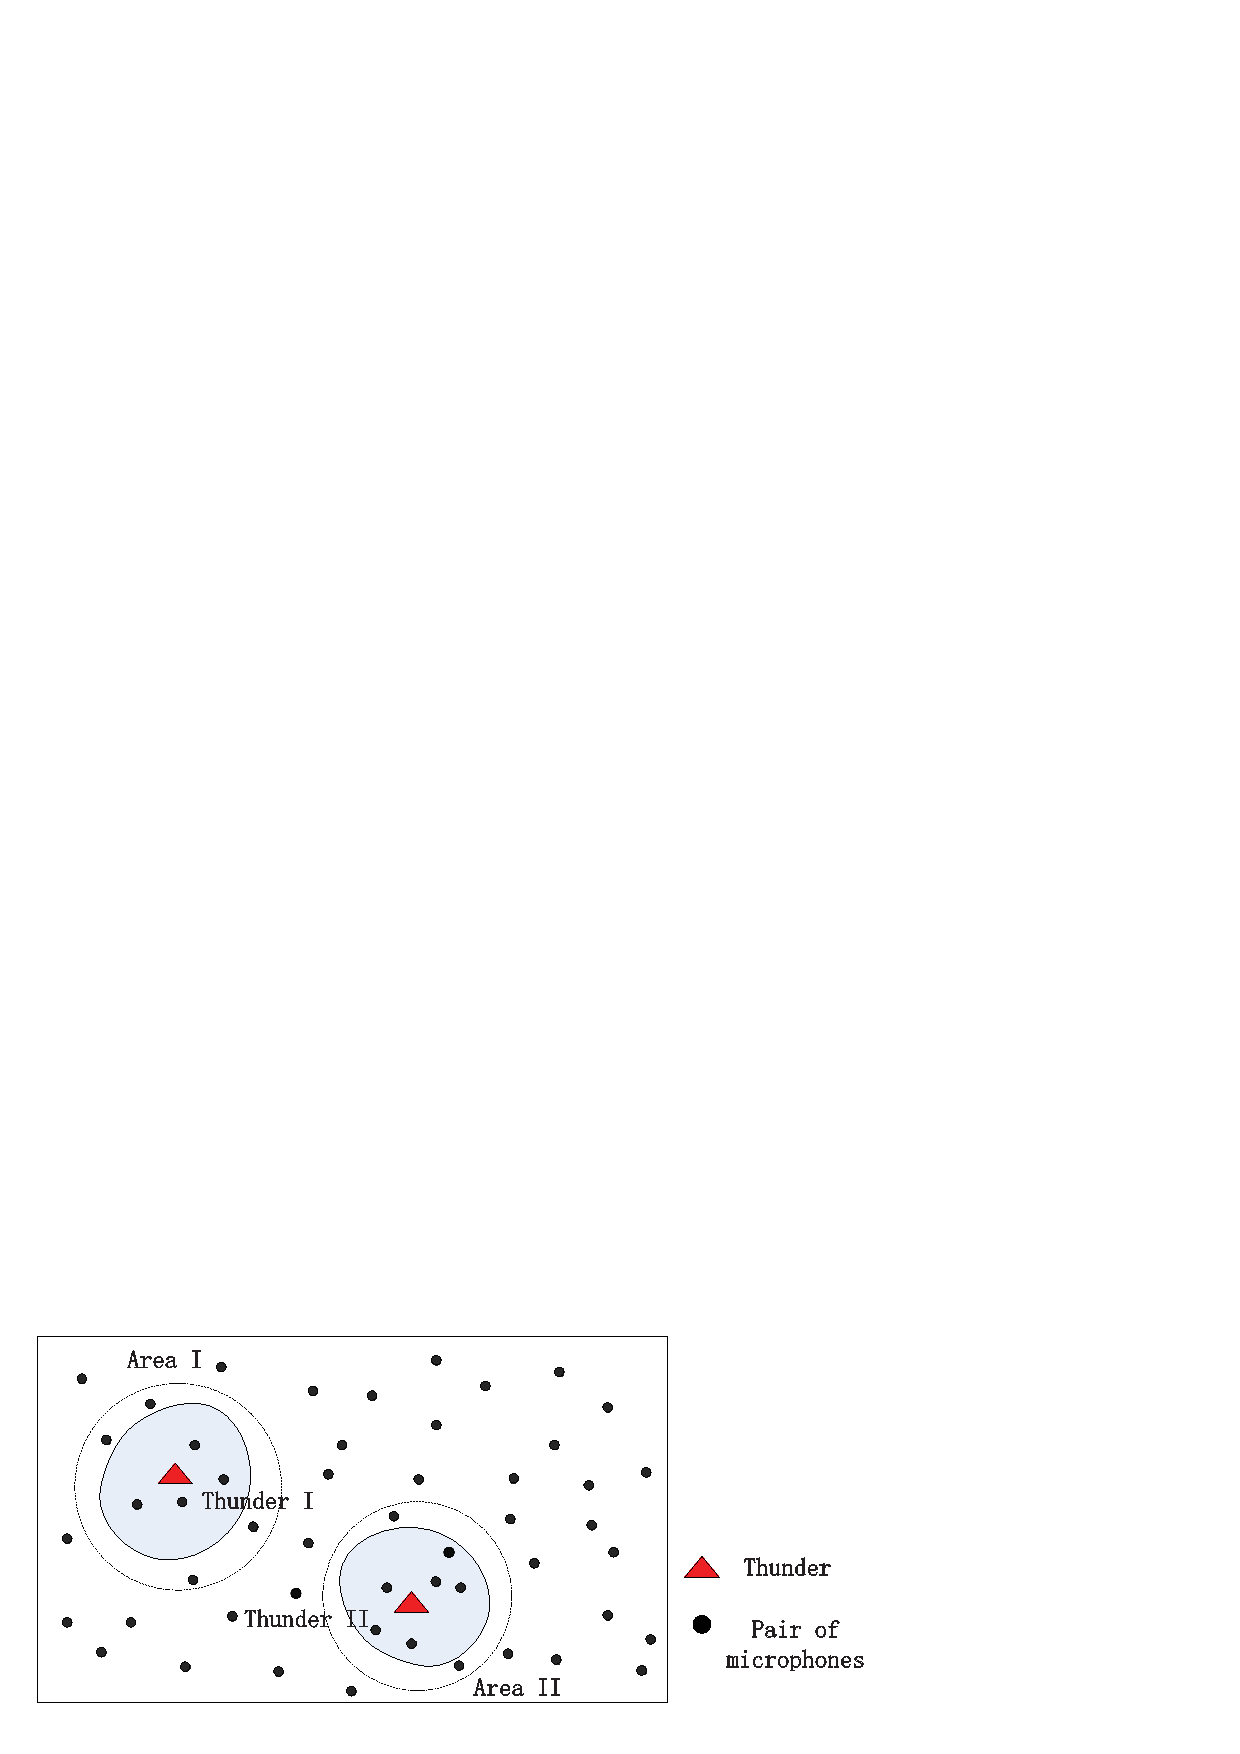
\includegraphics[scale=1.2,height=3.2cm]{fig/msl.pdf}
             \vspace{1mm}
			\caption{\label{Fig9:} System scalability for large-scale systems.}
            \label{multiple_source_localization}
            \vspace{-1mm}
  \end{figure}

 \vspace{-8mm}
 
\subsection{Time Synchronization and Energy Efficiency}
In our system, we calculate the sign of TDOA by utilizing two synchronized audio signals from dual-microphone of each smartphone. 
%Time synchronization among smartphones is not in high demand to locate the thunder, which is already supported in the recent 4G cellular network.
High-accuracy of time synchronization among smartphones is not required.

Energy efficiency is another issue in smartphone networks.
We can activate the ThunderLoc app in the smartphone according to the thundershower alert from the weather forecast app.
Only if it is raining with thunder, ThunderLoc app will be awake.








\section{Results}
\label{section:results}
% In the simulation, the distance between dual-microphones is 14cm, and audio sampling rate is 48kHz. 
% All the statistics are run more than 3000 times for high confidence, and reported by Root Mean Square Error (RMSE).
% The parameter $\sigma$ in robust ThunderLoc has little impact to the localization performance. In default, $\sigma=1$.
\subsection{2D Simulation}
In this section, we evaluated our localization methods in 2D scenario using MATLAB.  
In the simulation, we randomly deployed dual-microphone mobile phones on a 10km $\times$ 10km area with uniform distribution, and the distance between dual-microphones is 14cm, and audio sampling rate is 48kHz. 
All the statistics are run more than 3000 times for high confidence, and reported by Root Mean Square Error (RMSE).
The parameter $\sigma$ in robust ThunderLoc has little impact to the localization performance. In default, $\sigma=1$.
We intend to make a comprehensive assessment and comparison for the two proposed localization methods from different aspects, 
including the impact of the number of nodes, the number of fault nodes, the impact of the position error of nodes, the impact of the angle error of nodes. 
In default, there are 100 mobile phones and just one thunder. 
To simulate the impact of the position and orientation of smartphone nodes on the accuracy of localization, 
all the simulations are added a certain amount of position and angle error. 
%The unit of the angle error range is degree, and the position error range is meter. 
In default, the angle error range is 5 degree and the position error range is 100m. 
The results of simulation evaluation are as follows.

\textbf{1) Impact of the number of nodes:}
In this experiment, we investigate the localization error over number of nodes from 50 to 250 in steps of 10. 
We run the simulation with 2 samples TDOA error, and other simulation parameters are default. 
As shown in Fig. \ref{Node_Number}, with the increasing of the number of mobile phones, the whole area could be divided into more grids, thus more accurate localization estimation were achieved for both of two localization methods. 
When the number of mobile phones is low, the performance of robust ThunderLoc is better than basic ThunderLoc. 
With the increasing of the number of participants,  two localization methods could get almost the same localization performance.
  
 \textbf{2) Impact of the number of error nodes:}
In the practical application, if dual-microphone is very close to each other along the direction of event propagation, they
would detect the event almost simultaneously. In this case, the binary left/right data in the sequence may occur to flip. 
We called this smartphone as the error node.
In this experiment, we try to compare the two methods with different percentage of error nodes, and it ranges from 0 to 0.2 in steps of 0.01. 
Other simulation parameters remain default. The Fig. \ref{Faulty_Node} indicates that the localization error increases as the number of error nodes increases for both of the two methods. 
And it also shows as the number of error nodes increases, the average localization error of robust ThunderLoc is little smaller than that of basic ThunderLoc.
robust ThunderLoc provides a effective solution to deal with the bit flip problem mentioned before.
  
 \textbf{3) Impact of the position error of nodes:}
In the experiment, we evaluated the impact of the position error of nodes for the basic ThunderLoc and robust ThunderLoc with the range from 0 to 1000m in steps of 50. 
Other simulation parameters keep default. Fig. \ref{Location} shows that with the increasing of the position error of smartphone nodes, the average localization error of robust ThunderLoc is much smaller than that of basic ThunderLoc.

    \begin{figure}[hptb]
            \setlength{\abovecaptionskip}{0pt}
            \centering
            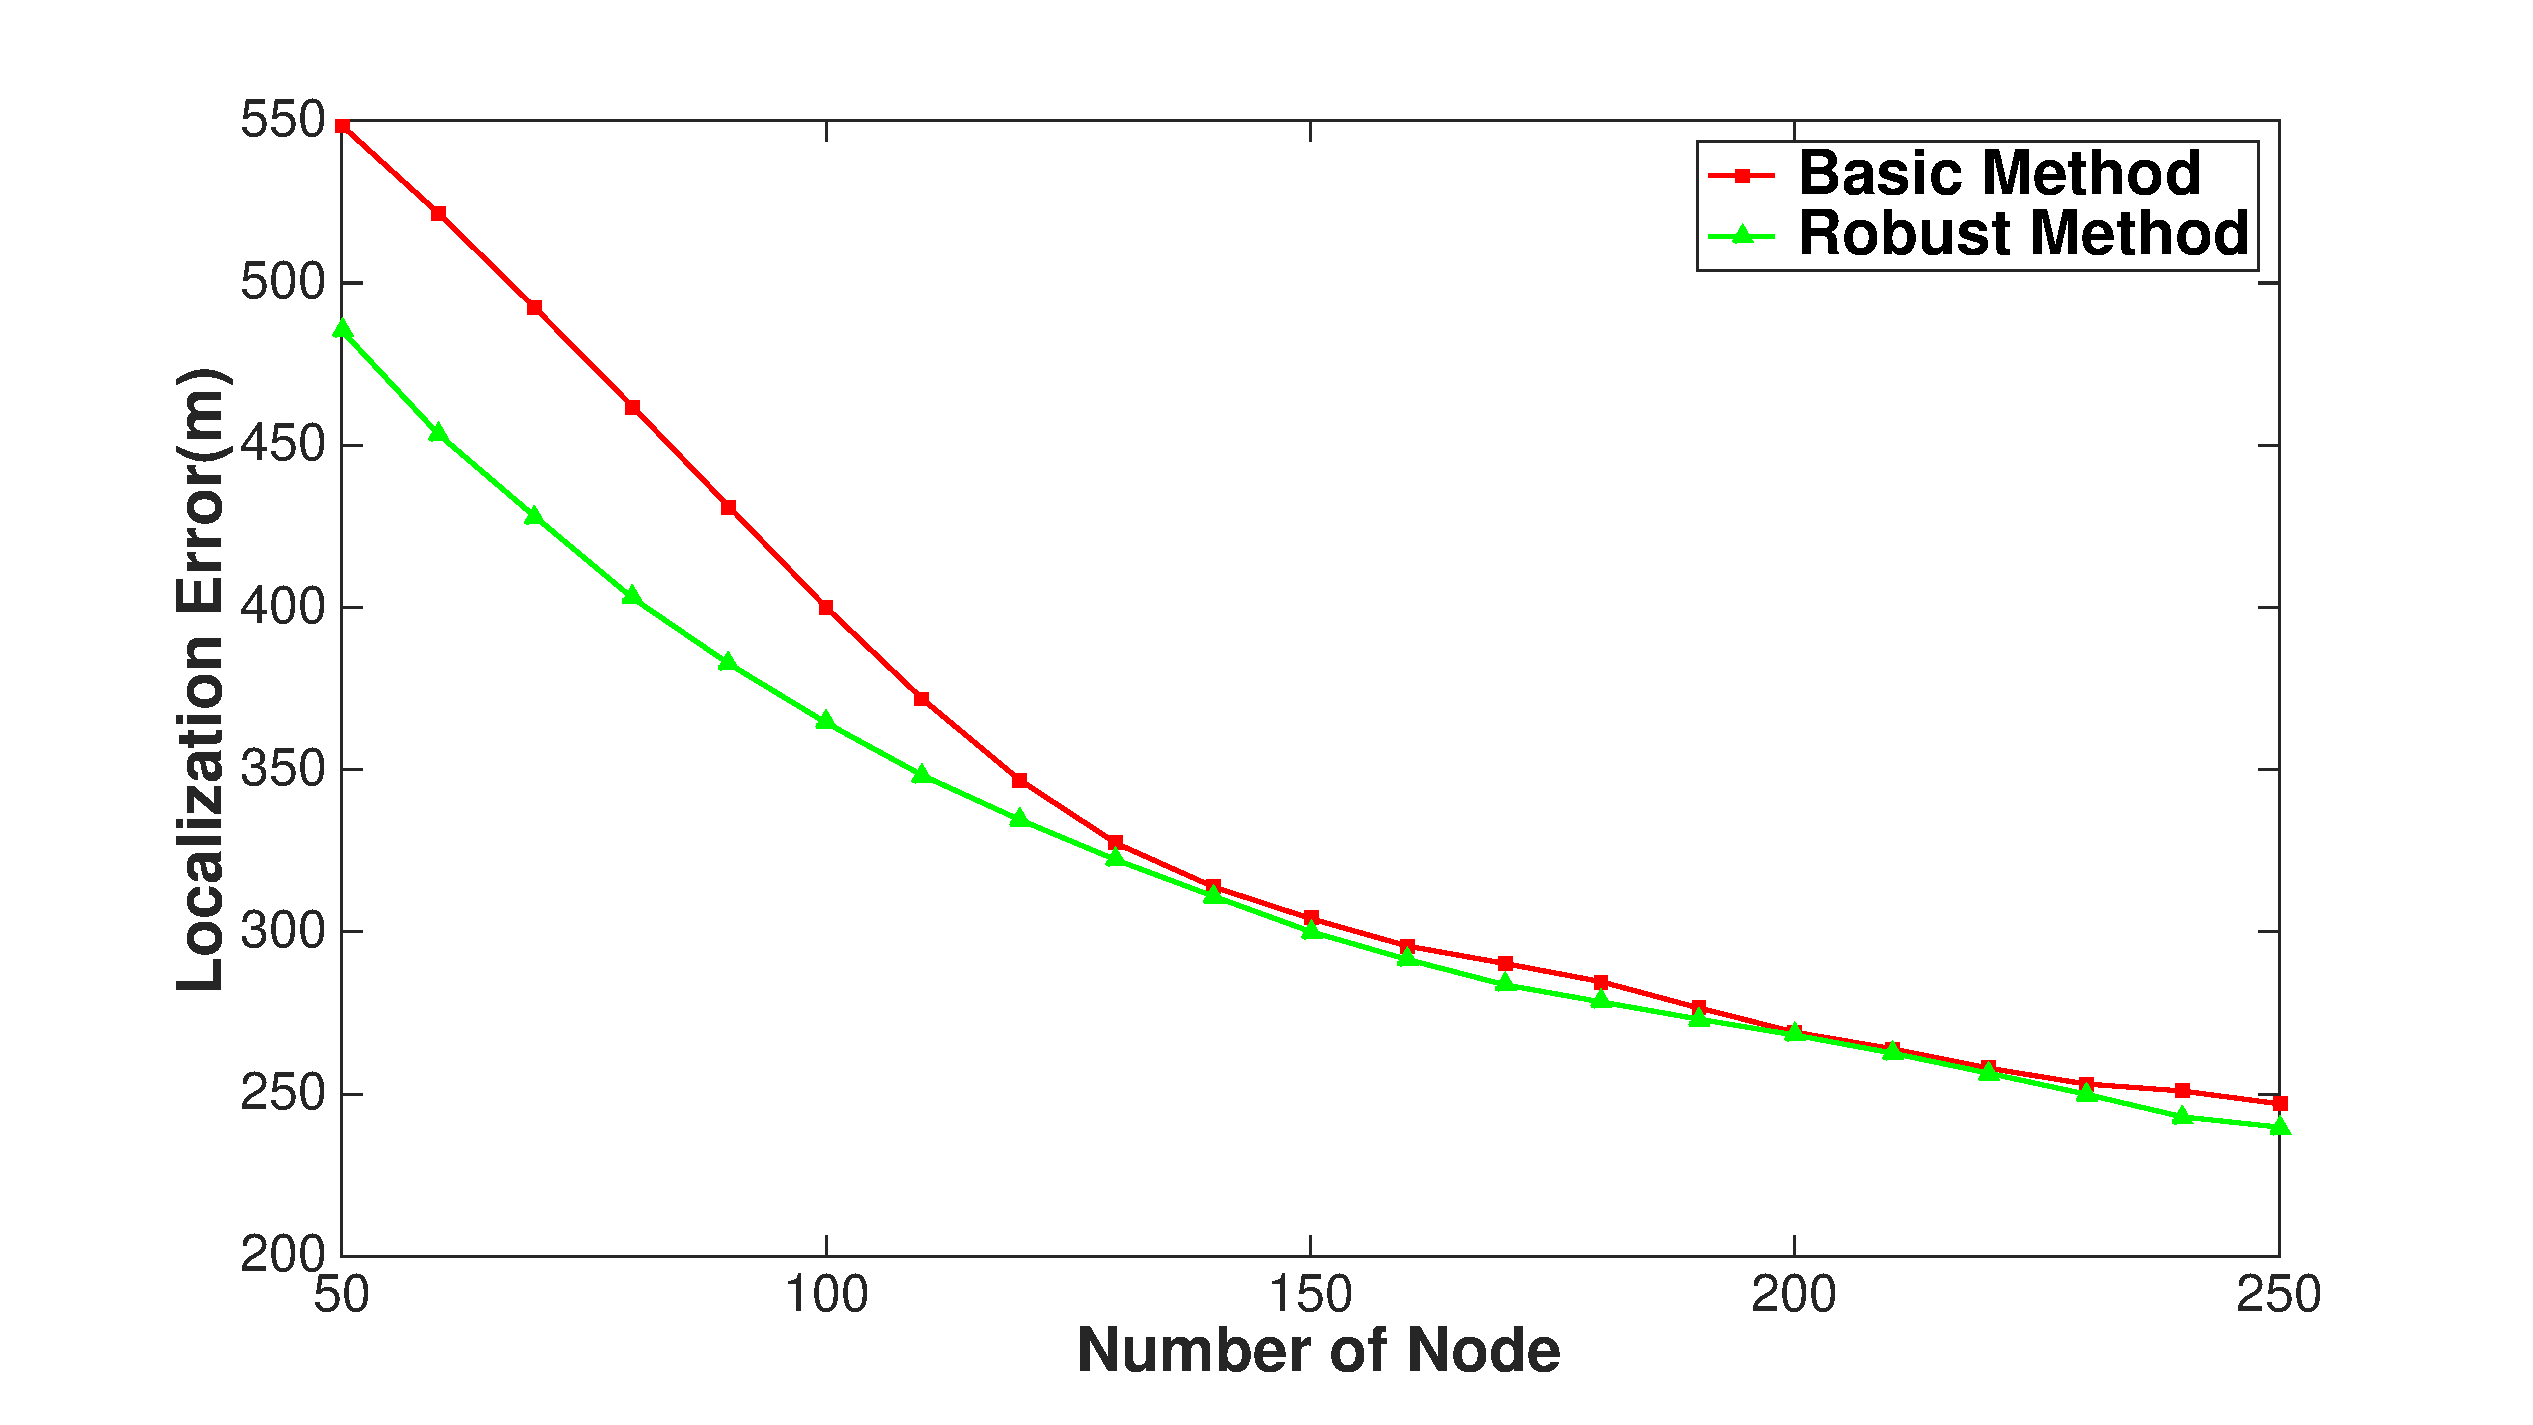
\includegraphics[scale=1.4,height=4.0cm]{image/Node_Number.eps}
     \vspace{2mm}
            \caption{Impact of number of nodes}
            \label{Node_Number}
            \vspace{-6mm}
  \end{figure}

\begin{figure}[hptb]
            \setlength{\abovecaptionskip}{0pt}
            \centering
            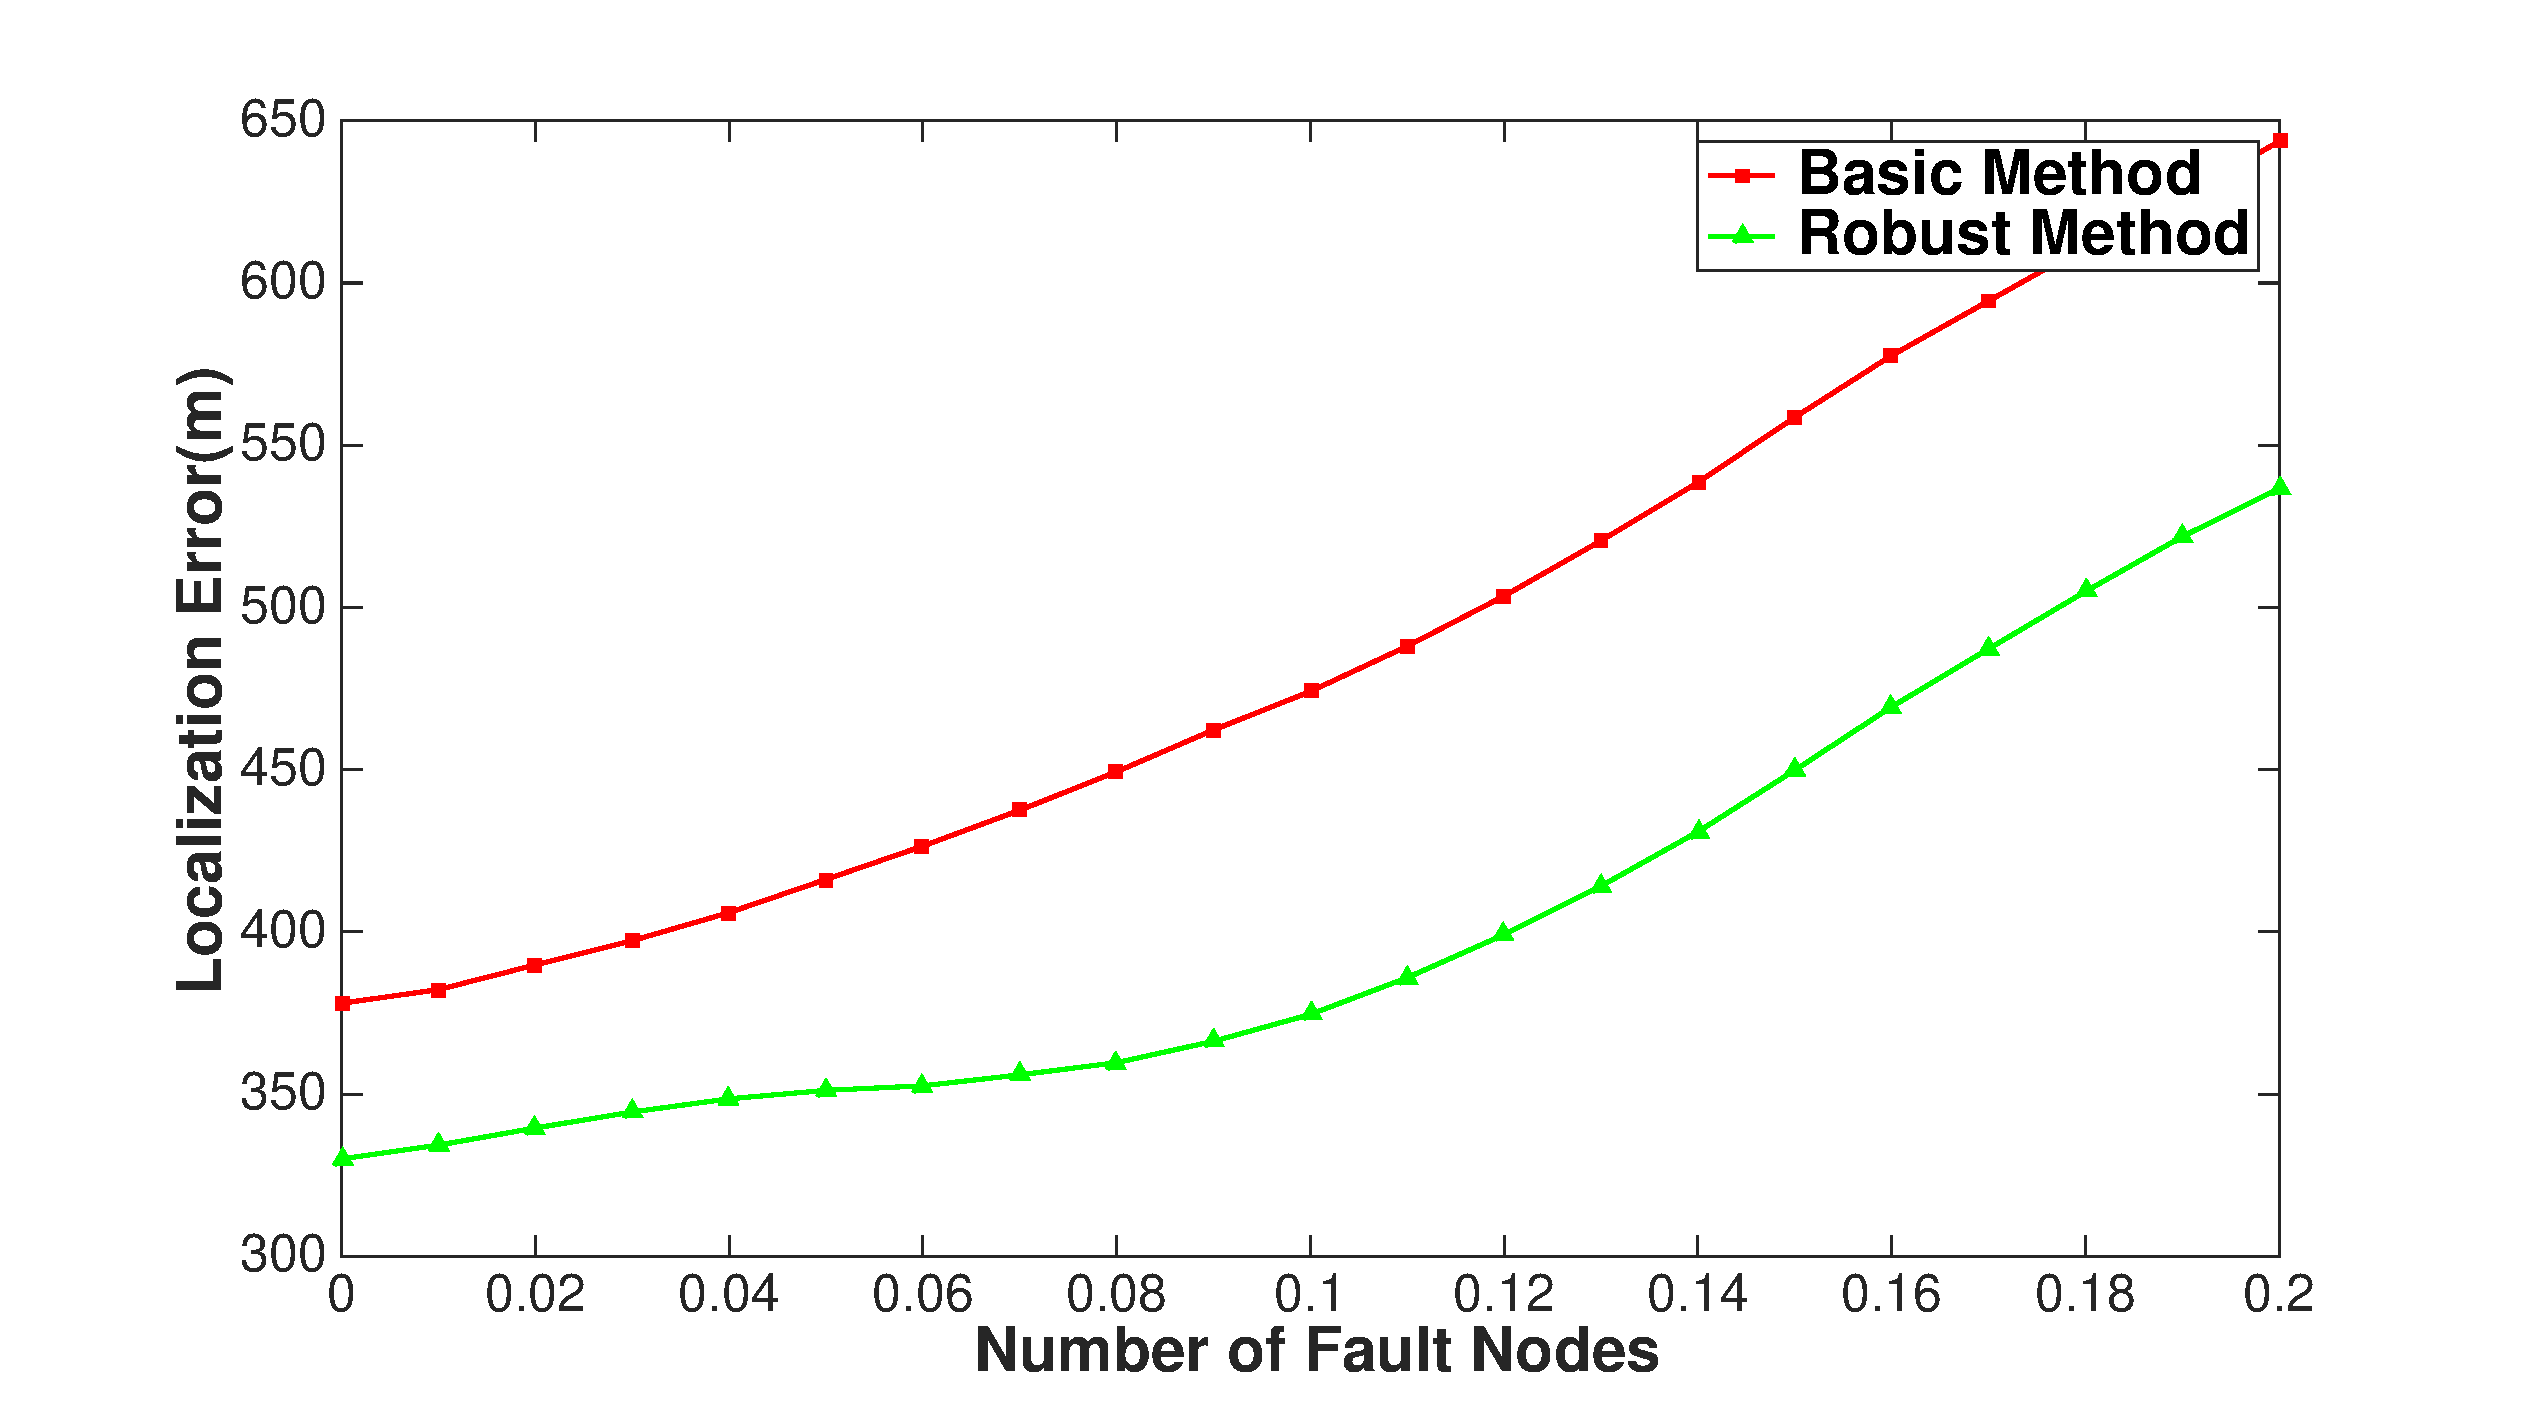
\includegraphics[scale=1.4,height=4.0cm]{image/Faulty_Node.eps}
     \vspace{2mm}
            \caption{Impact of number of error nodes.}
            \label{Faulty_Node}
            \vspace{-6mm}
  \end{figure}

  \begin{figure}[hpt]
            \setlength{\abovecaptionskip}{0pt}
            \centering
            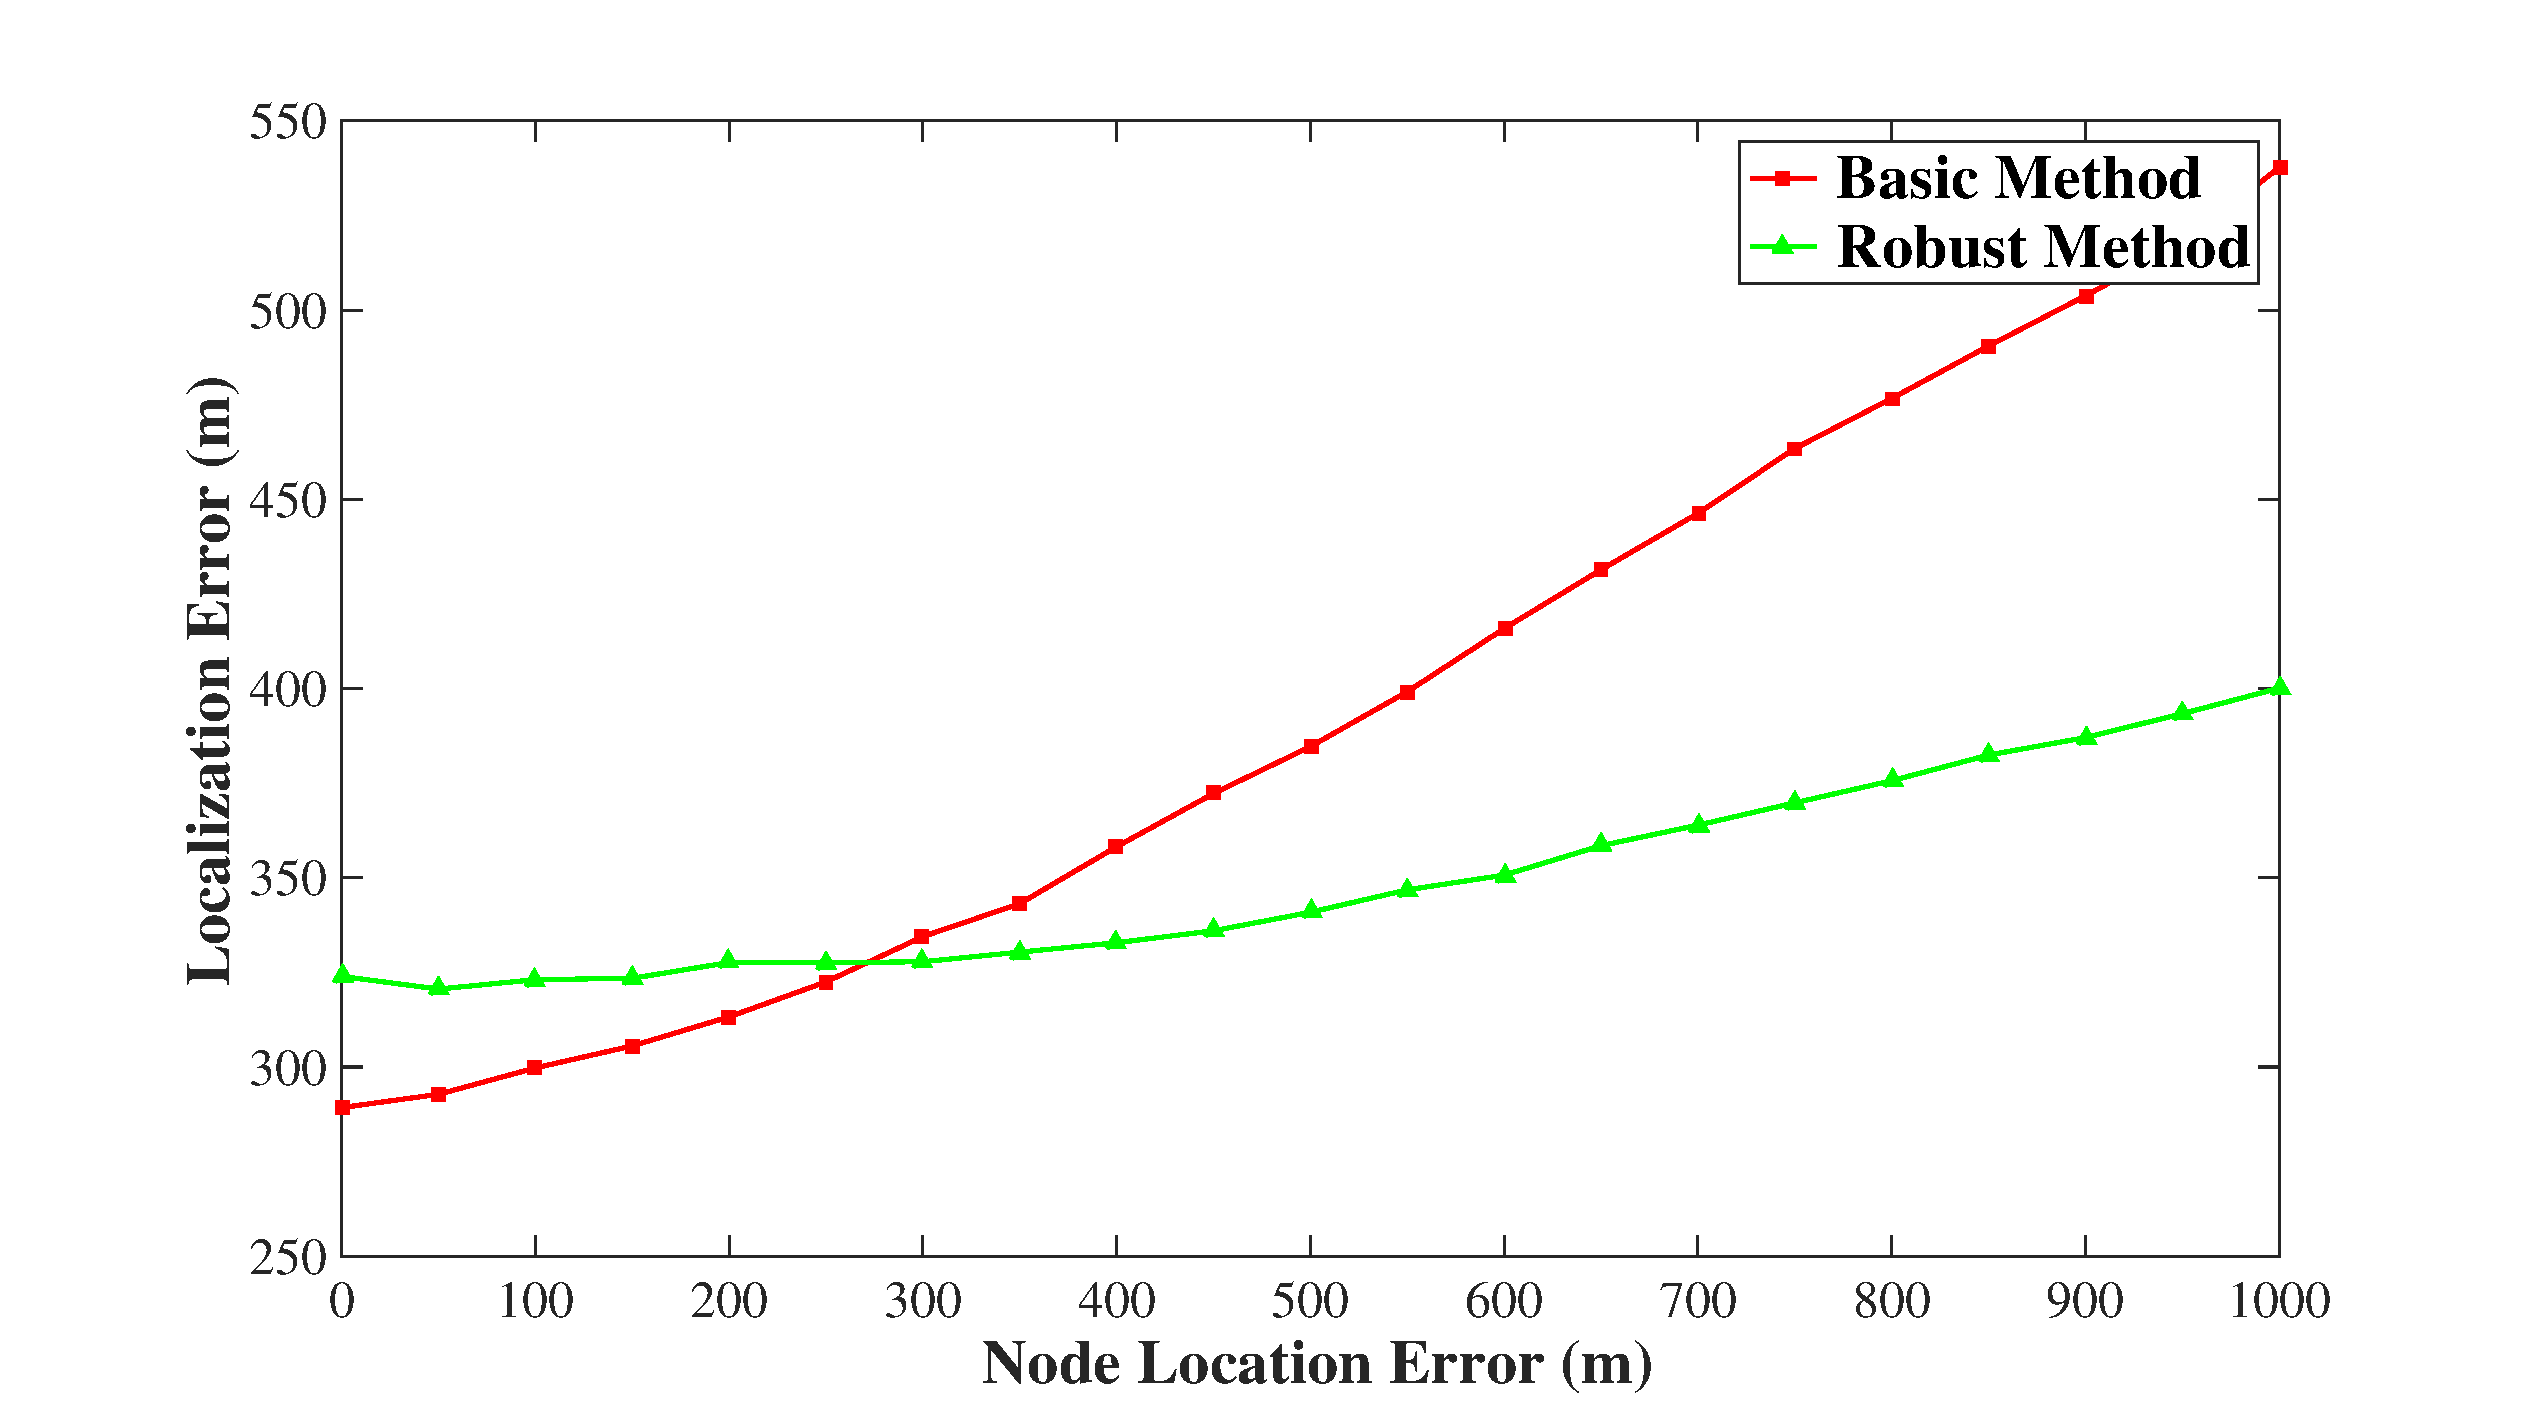
\includegraphics[scale=1.4,height=4.0cm]{image/Location.eps}
     \vspace{2mm}
            \caption{Impact of the position error.}
            \label{Location}
            \vspace{-6mm}
  \end{figure}
  
  \textbf{4) Impact of the orientations error of nodes:}
In the experiment, we evaluated the impact of the angle error of nodes for the basic ThunderLoc and robust ThunderLoc with the range from 0 to 20 degree in steps of 2. 
Other simulation parameters keep default.
As the orientations of nodes exist errors, we can guess the error of orientations may influence the localization accuracy. 
 As shown in Fig. \ref{Direction}, the graph to the localization error for the two methods is rising as the angle error of nodes increases. 
When the angle error of nodes is relative large, the average localization error for the robust ThunderLoc is much smaller than basic ThunderLoc, 
 so the localization accuracy of robust ThunderLoc is much better than that of basic ThunderLoc.
  \begin{figure}[hptb]
            \setlength{\abovecaptionskip}{0pt}
            \centering
            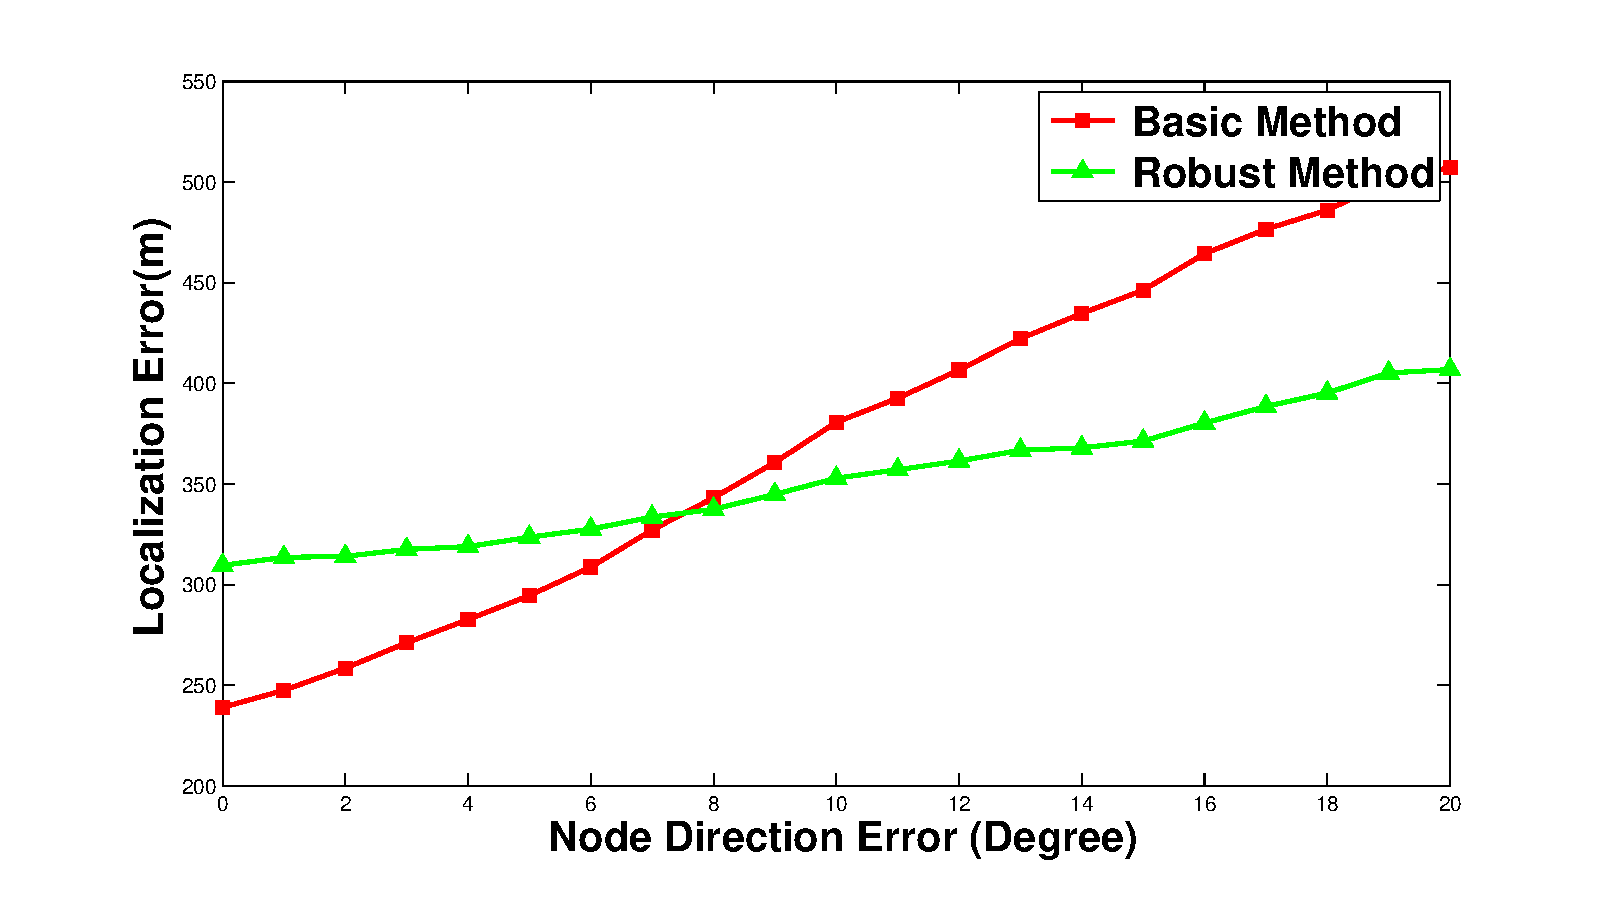
\includegraphics[scale=1.4,height=4.0cm]{image/Direction.eps}
     \vspace{2mm}
            \caption{Impact of orientation error.}
            \label{Direction}
            \vspace{-6mm}
  \end{figure}

 

 % \textbf{Summary:} From these experiments, we can get the following conclusions:

 % (1) The increase of the number of nodes can improve the localization accuracy, especially when we have many participants holding the mobile phones with different postures.

 % (2) The increase of the number of fault nodes can reduce the localization accuracy, and robust ThunderLoc is better than basic ThunderLoc when the percentage of fault nodes is above 0.06.

 % (3) The errors of node position and orientation can impact the localization error, the localization performance of robust ThunderLoc is better than basic ThunderLoc.

  \vspace{-4mm}
\subsection{3D Simulation}

The height of the thunder should be considered in some applications, such as lightning channel reconstruction. 
In this section, we evaluated our localization methods in the 3D scenario.  
In the simulation, we randomly deployed 100 dual-microphone smartphones to cover a 10km $\times$ 10km region. 
The altitude of mobile phones is about 10m and the height of the thunder is about 3km. 
The number of nodes is 100, and the angle error range of smartphones is 5.
Due to limitations on space, we just investigate the impact of the number of smartphones with the range from 80 to 160. 
The localization result of the experiment is showed in Fig. \ref{3D}.
Comparison with the 2D scenario, the localization errors are much larger in 3D space for the same number of smartphones. 
The reason is that the localization errors are related to the size of space grids divided by the perpendicular bisector of dual-microphone.
In the 3D scenario, the more smartphones is needed to achieve high-accuracy localization. 
%When the number of nodes is 120, the average localization error of robust ThunderLoc is about 800m.
  \begin{figure}[ht]%HT
            \setlength{\abovecaptionskip}{0pt}
            \centering
            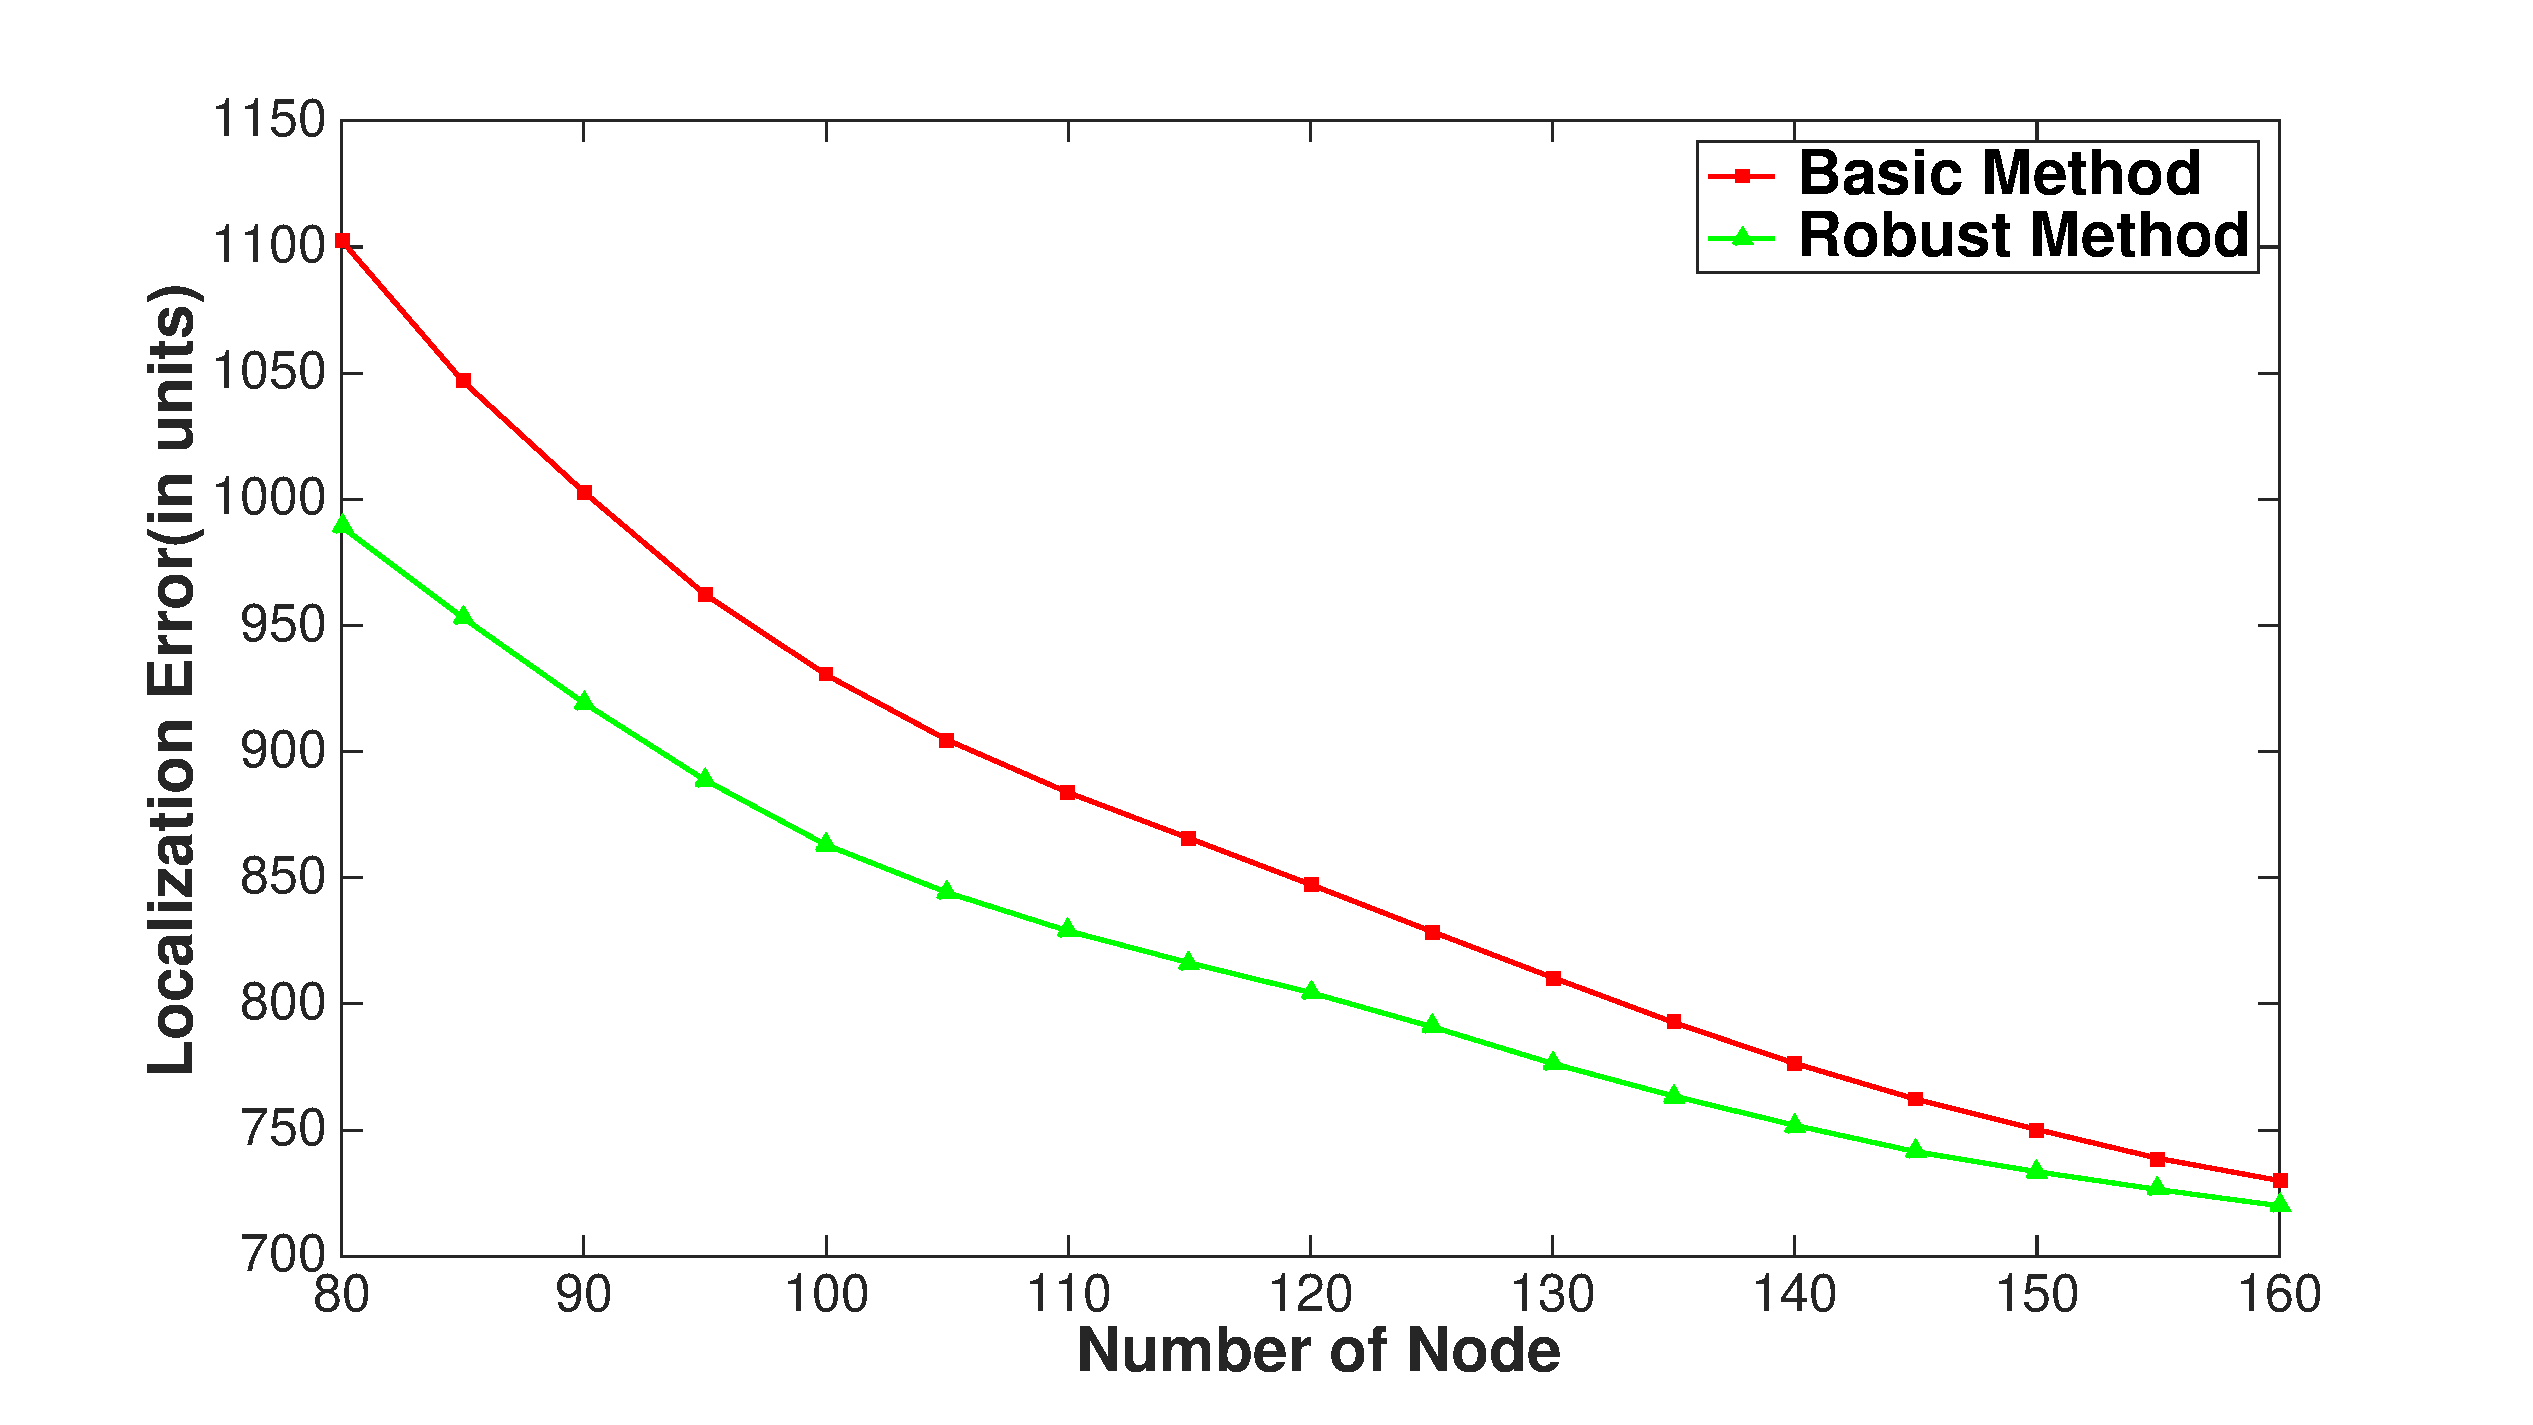
\includegraphics[scale=1.4,height=4.0cm]{image/3D.eps}
     \vspace{2mm}
    	   \caption{Thunder localization in 3D space}
            \label{3D}
            \vspace{-6mm}
  \end{figure}
  
\subsection{Virtual Thunder Emulation}

The virtual thunder test was useful as a proper verification of the functionality of our ThunderLoc project. 
We use 30 dual-microphone Xiaomi smartphones as sensor nodes and connect them through CISCO CVR328W-K9-CN wireless router. 
The distance between the two microphones is 14cm. We set the 30 nodes in a size of 1km$\times$1km space and there just one target during an experiment.
In order to simulate the thunder, we broadcast the recorded sound signal of thunder by speaker at the top of the three buildings. 
Smartphones are randomly deployed around the building.The localization results are shown in Fig. \ref{Virtual}, where blue squares stand for dual-microphone smartphones, and blue circles and red circles are the ground truth and the estimated position by robust localization method. 
An arrow originates from the estimated position to the real position of the virtual thunder. 
As the results shown in Fig. \ref{Virtual}, the estimated position is close to real position and the localization error is within the expected range,
which means that our proposed ThunderLoc system can effectively locate the thunder  by the way of crowdsensing.
  \begin{figure}[ht]
            \setlength{\abovecaptionskip}{0pt}
            \centering
            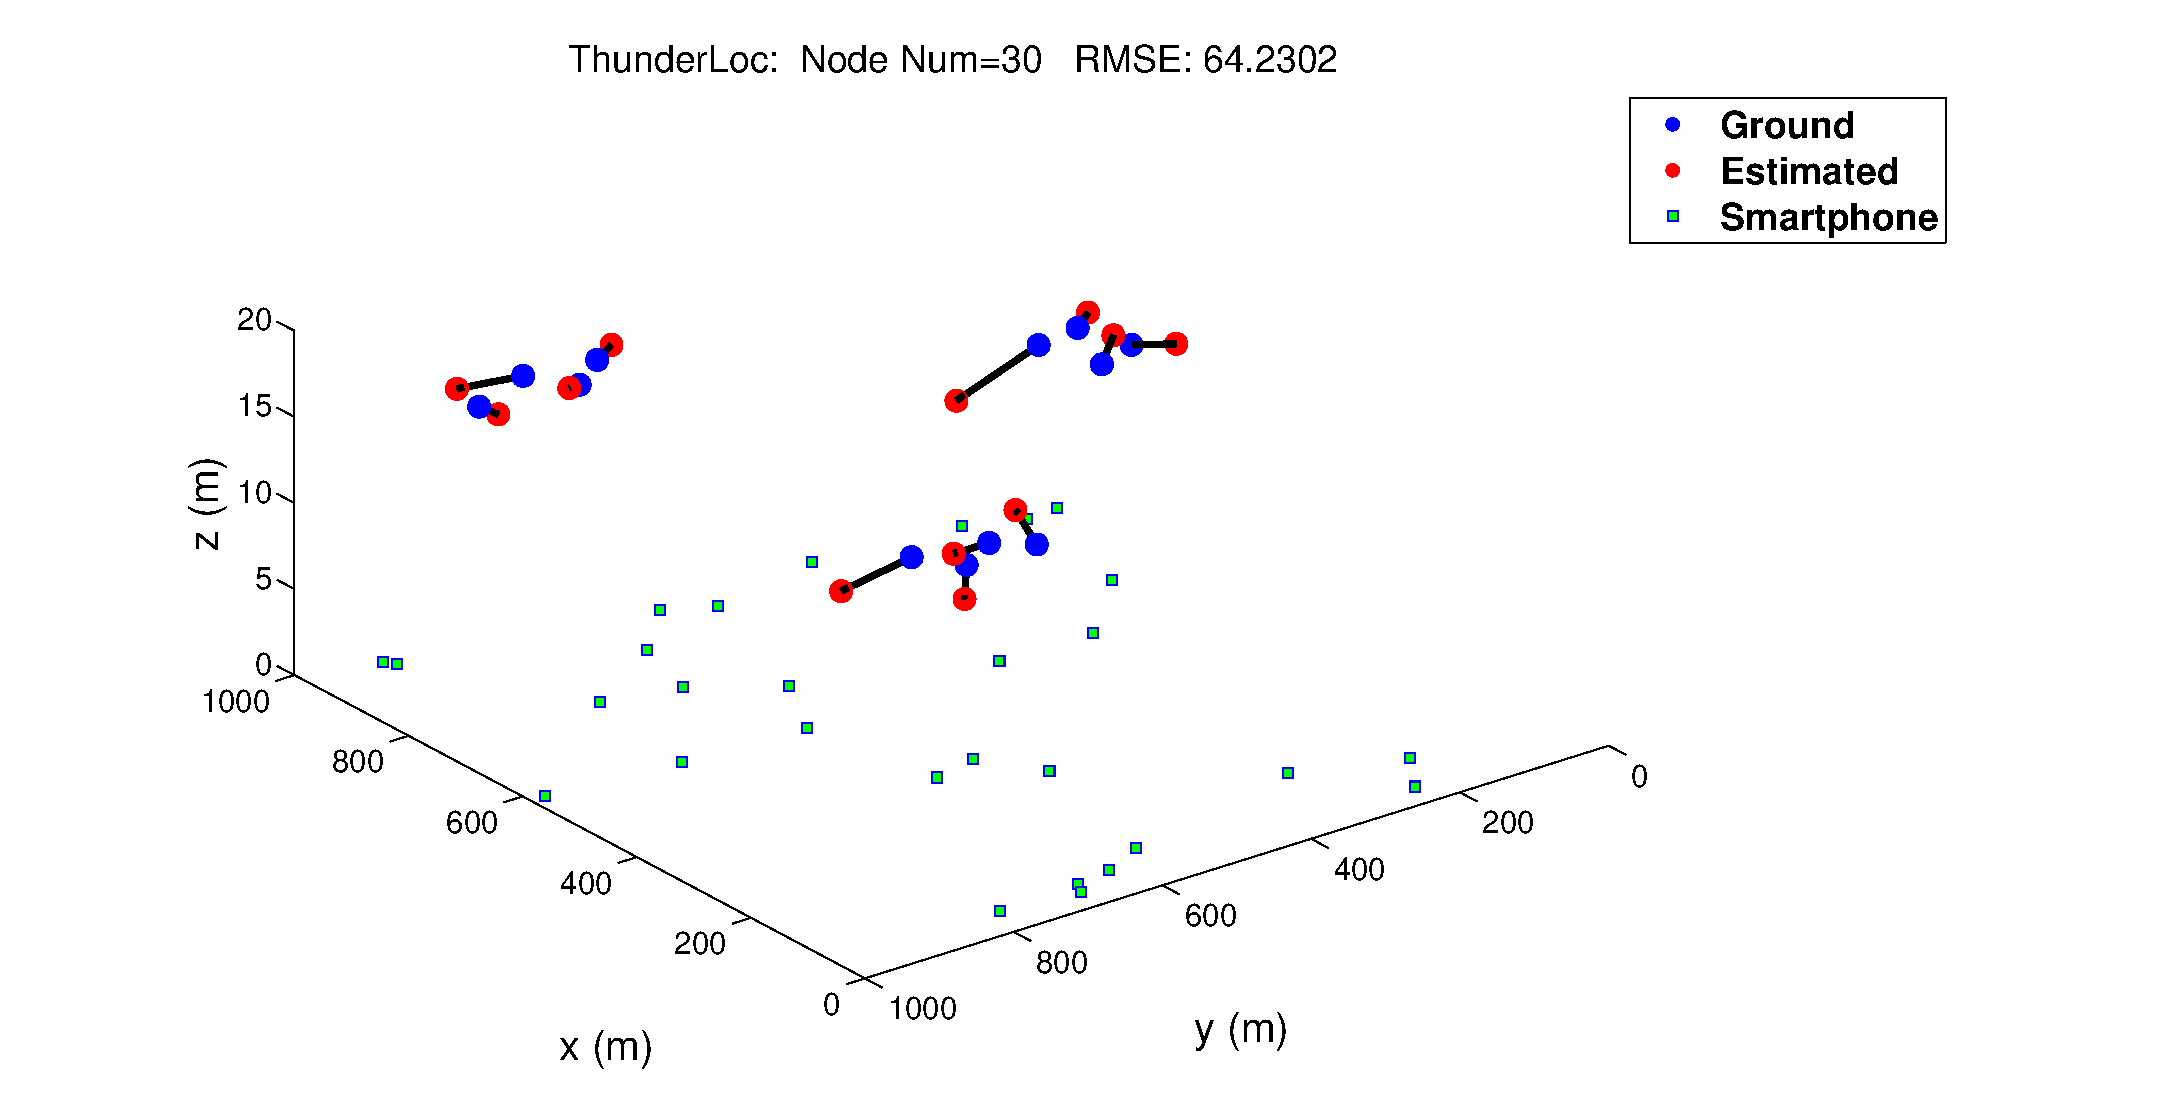
\includegraphics[scale=2,height=4.5cm]{image/virtual.eps}
     \vspace{2mm}
            \caption{Experiment result.}
            \label{Virtual}
            \vspace{-8mm}
  \end{figure}




\section{Related Work}


%Based on the high position accuracy of the LMA (6�C12 m RMS in the horizontal and 20�C30 m RMS in the vertical for sources over the network) [ Thomas et al. , 2004 ], it can be used as
%reference (ground truth) to investigate the position accuracy of the acoustic array.
% Audible thunder (great than 20 Hz,3.3 to 500 Hz)
%: A major challenge for the early TOA systems was the need for precise time synchronization of multiple remote sensors.

%As a case study of acoustic source localization technology, 

% Lightning@SG, an App developed by National Environment Agency (NEA) that provides current lightning situation in Singapore, which uses lightning information from the latest lightning detection and location system to locate lightning. 
% It has four lightning detection sensors located in four cities.

%Thunder localization has drawn more attention for lightning location systems in recent years.
%According to the different frequency, 
Thunder localization system can use infrasonic signals, supersonic signals, and audible signals as the measurement data.
Due to space constraints, we can only mention a few related works using audible sound data.
%Audible thunder is thought to come from the expansion of the rapidly heated lightning channel.
Most of the existing thunder localization systems using audible sound data are based on centralized architecture.
Arechiga, \emph{et al.} \cite{arechiga2011acoustic} studied acoustic reconstruction of lightning channel geometry using microphone arrays, improved upon thunder localization by using compact acoustic arrays with 1kS/s sample rate.
Akiyama, \emph{et al.} \cite{akiyama1985channel} used rhombus array with 100k sample rate and 3.50m base line.
Few, \emph{et al.} \cite{few1970lightning} implemented lightning channel reconstruction using 'Y' 4-element array with 1k sample rate and 30m base line.
MacGorman, \emph{et al.} \cite{macgorman1978lightning} considered the effect of temperature and wind, presented a lightning localization system with square array with 0.5k sample rate and 50m base line.
Johnson, \emph{et al.} \cite{johnson2011imaging}  used a network of broadband microphones, including a 4-element array with 1k sample rate, to locate the sources of thunder occurring during an electrical storm.
Qiu, \emph{et al.} \cite{qiu2012synchronized}  used 3-element array with 100k sample rate and 12.5m base line to estimate the location of thunders.


In the past few years, there has been a growing interest for acoustic localization based on independent (unsynchronized) acoustic sensors, each made of two or more synchronized microphones. 
UbiK leveraged the dual-microphone on a mobile device to accurately localize the keystrokes \cite{UbiK}.
Zhu, \emph{et al.} \cite{Zhu2014Context} proposed to utilize dual-microphone on three phones to identify keystrokes of a nearby keyboard based on
time difference of arrival (TDOA) measurements.
Liu, \emph{et al.}  \cite{Liu2015Snooping}  achieved keystroke recognition by discriminating keystrokes based on TDOA of the keystroke sound at the dual-microphone of the off-the-shelf smartphone.
Wang, \emph{et al.} \cite{wang2003acoustic} described a system having static cluster architecture, the system experienced a problem in that the accuracy decreased when an acoustic source occurred between the clusters.
Chen, \emph{et al.} \cite{chen2004dynamic} showed that nodes in the system did not need to recognize their cluster head, reducing the constraints on deployment of the localization system.
Hu, et al. \cite{hu2009design} design the system based on 2-tier architecture, which experienced cost and deployment problems especially in the very large target area.
%Rabbat, \emph{et al.} \cite{rabbat2005robust} proposed a decentralized algorithm based on the distributed ML estimation technique using token ring architecture.
%Kim, \emph{et al.} \cite{kim2009locating} proposed to identify the node closest to the acoustic source, based on TOA comparisons between all nodes, thus incurring high communication cost and requiring global synchronization between all sensor nodes.
% Lightning is a method proposed in \cite{wang2008lightning} to identify the sensor closest to the acoustic source, also based on expensive broadcasting/flooding.
%Aarabi, \emph{et al.} ~\cite{aarabi1900fusion} used 10 dual-microphone arrays distributed in a room and used their data to locate three speakers.
%Wu, \emph{et al.} ~\cite{wu2012fusion} used three dual-microphone arrays to locate two sound sources in a distributed way in which only the local DOA estimates are communicated among arrays.
Canclini, \emph{et al.}\cite{canclini2013acoustic} proposed a method for localizing an acoustic source with distributed microphone networks based on TDOA between microphones of the same sensor. 
%Most of the existing acoustic source localization methods in sensor networks are based on range-based measurement.
%In contrast, 
Different from these range-based methods, 
our proposed ThunderLoc is a range-free method, which can achieve robust localization performance.

The most related work to our ThunderLoc project is Lightning@SG, an App developed by National Environment Agency (NEA) in Singapore~\cite{LightningSG}. 
By utilizing the four sensors located in different cities, Lightning@SG monitors the lightning area based on current location of user, and pushes notifications of the lightning situation.
With the surging of smartphone sensing and wireless networking techniques,
crowdsensing has become a promising paradigm for cross-space and large-scale sensing. The iShake system uses smartphones as seismic sensors to measure and deliver ground motion intensity parameters produced by earthquakes~\cite{reilly2013mobile}.
Hu, \emph{et al.} presented SmartRoad, a crowd-sourced road sensing system that detects and identifies traffic regulators, traffic lights, and stop signs~\cite{hu2013smartroad}.  
Zhou, \emph{et al.} presented  a novel bus arrival time prediction system based on crowd-participatory sensing~\cite{zhou2012long}. 
Motivated by these works, we uses dual-microphone smartphones as sensors to estimate the position of the thunders by crowdsensing mechanisms.


\section{Conclusions and Future work}

In this paper, we have designed DroneLoc, a novel drone localization system that leverages  smartphones to achieve drone localization using unreliable detection data by deep neural network.
The proposed design formulates the drone localization as the searching problem  by making use of the data from the smartphones.
Since our DroneLoc system runs on COTS smartphones and supports spontaneous setup, it has potential to enable a wide range of drone localization systems.
Besides the basic design, a robust localization method is proposed to enhance the localization performance in the practical application.
Our system is verified and evaluated through analysis, extensive simulation as well as the test-bed experimentation.
The test results have shown that the proposed method can effectively implement drone localization with smartphone camera networks.
Our next step is to study the distributed implement of the proposed DroneLoc.


% \section{Acknowledge}

% This work is supported by Natural Science Foundation of China (Grants No. 61272524 and No.61202443) and the Fundamental Research Funds for the Central Universities (Grants No.DUT15QY05 and No.DUT15QY51).
% This work is also supported by Specialized Research Fund for the Doctoral Program of Higher Education (Grant No. 20120041120049).



\bibliographystyle{IEEEtran}
\bibliography{Main}

\end{document}
